\documentclass[11pt]{article}
\usepackage[a4paper,margin=1in]{geometry}
\usepackage{amsmath,amssymb,bm}
\usepackage{graphicx}
\usepackage[hypertexnames=false]{hyperref}
\usepackage{booktabs}
\usepackage{float}
\usepackage[section]{placeins}
\usepackage{array}
\usepackage{adjustbox}
\usepackage{algorithm}
\usepackage{algpseudocode}
\setlength{\emergencystretch}{1.5em}
\algrenewcommand\algorithmicrequire{\textbf{Input:}}
\algrenewcommand\algorithmicensure{\textbf{Output:}}

\newcommand{\q}{\mathbf q}
\newcommand{\qbar}{\overline{\mathbf q}}
\newcommand{\qtot}{\mathbf q_{\mathrm{tot}}}
\newcommand{\qp}{\q}
\newcommand{\qs}{\qbar}
\newcommand{\uvec}{\mathbf u}
\newcommand{\utilde}{\widetilde{\mathbf u}}
\newcommand{\mub}{\bm\mu}
\newcommand{\z}{\mathbf z}
\newcommand{\norm}[1]{\left\lVert #1 \right\rVert}
\newcommand{\papertable}[1]{%
  \begingroup
  \small
  \setlength{\tabcolsep}{3.5pt}%
  \renewcommand{\arraystretch}{1.15}%
  \begin{adjustbox}{max width=\textwidth}
  \input{#1}
  \end{adjustbox}%
  \endgroup
}

\title{\vspace{-1.5em}Neural closures in nonlinear projection-based model reduction: Comparative assessment and residual-adaptive correction}
\author{S. Ares de Parga, H. Ballout, Y. Maday}
\date{\today}

\begin{document}
\maketitle
\vspace{-1.0em}
\begin{center}
\small\emph{Alternative title: Residual-adaptive correction of neural closures for projection-based model reduction: Formulation and comparative assessment}
\end{center}
\vspace{-1.0em}

\begin{abstract}
Nonlinear trial manifolds offer a way to mitigate the Kolmogorov barrier
to linear reducibility.  Neural-network-augmented projection-based
reduced-order models (PROM--ANN) determine primary reduced coordinates
through residual minimization and reconstruct secondary coordinates
through a learned closure.
The usual state-conditioned closure (Case~1) assumes that primary
coordinates uniquely determine secondary coordinates, which need not hold
globally.  We examine two alternatives: conditioning on parameters and
time alone (Case~2), or jointly on primary coordinates, parameters, and
time (hybrid Case~3).  Case~2 has a fixed trial tangent and requires no online
derivatives of the network, reducing computational cost.  However, its
residual solve cannot adjust the prescribed secondary coordinates,
potentially limiting accuracy.  We introduce a residual-adaptive
correction that selects a few directions in the secondary-coordinate
space and determines their amplitudes together with the primary
coordinates.  The correction uses the governing residual and Jacobian
without retraining the network or adding training trajectories.

On a two-dimensional parametric Burgers benchmark, we compare hyperreduced
projection-based models (HPROM--ANN and HPROM--POD--AE) with nonintrusive
POD--NN--ROM and POD--DL--ROM
maps, and assess training-data enrichment.  In the nine-trajectory
comparison, HPROM--ANN Case~2+$\mathbf B_3$ uses 13 online unknowns and
attains $0.454\%$ mean in-domain state
error relative to the high-dimensional model.  This is close to the
$0.441\%$ of the 151-coordinate linear HPROM and below the $0.553\%$ of
the conventional 10-coordinate state-conditioned HPROM--ANN (Case~1);
HPROM--ANN Case~2 gives $1.620\%$.  HPROM--ANN Case~2+$\mathbf B_3$ achieves an
observed $122\times$ speedup relative to the high-dimensional model,
corresponding to $12.5\times$ relative to the linear HPROM and $3.5\times$
relative to HPROM--ANN (Case~1).
\end{abstract}

\vspace{-0.8em}

\section{Introduction}
\label{sec:introduction}
\noindent\emph{Left blank for now.  The introduction and its literature
review will be completed in a later revision.  References currently cited
in the subsequent sections are preliminary; further references will be
added as those sections are developed.}
% Introduction note: place hernandez2026hyperreduction in the historical
% discussion of nonlinear coordinates.  It permits dense linear combinations
% of modal coefficients and includes a parameter-aligned limiting case in
% which the complete latent state is evaluated without a projected solve.

\section{Affine Projection-Based Model Order Reduction}
\label{sec:projection-framework}

\subsection{POD trial space}
Let $\uvec(t;\mub)\in\mathbb R^N$ denote the solution of the
high-dimensional model (HDM), with
$t\in[0,T_f]$ and $\mub\in\mathcal D\subset\mathbb R^p$.
From a collection of $N_s$ HDM
solution snapshots $\{\uvec^i\}_{i=1}^{N_s}$, define the reference state and
centered snapshot matrix
\begin{equation}
\uvec_{\mathrm{ref}}=\frac{1}{N_s}\sum_{i=1}^{N_s}\uvec^i,
\qquad
\mathbf S_c=
\begin{bmatrix}
\uvec^1-\uvec_{\mathrm{ref}} & \cdots &
\uvec^{N_s}-\uvec_{\mathrm{ref}}
\end{bmatrix}.
\label{eq:centered-snapshots}
\end{equation}
Proper orthogonal decomposition (POD) constructs an orthonormal basis by
compressing these centered snapshots.  Writing
$r_S=\operatorname{rank}(\mathbf S_c)$, the compact
singular-value decomposition (SVD) is
\begin{equation}
\mathbf S_c=\mathbf U_{\mathbf S}\boldsymbol\Sigma_{\mathbf S}
\mathbf Y_{\mathbf S}^T.
\label{eq:snapshot-svd}
\end{equation}
Here $\mathbf U_{\mathbf S}\in\mathbb R^{N\times r_S}$ and
$\mathbf Y_{\mathbf S}\in\mathbb R^{N_s\times r_S}$ have orthonormal
columns, and $\boldsymbol\Sigma_{\mathbf S}$ contains the positive singular
values $\sigma_1\geq\cdots\geq\sigma_{r_S}>0$.  A
standard energy criterion selects $n_{\mathrm{tot}}\ll N$ such that
\begin{equation}
1-\frac{\displaystyle\sum_{i=1}^{n_{\mathrm{tot}}}\sigma_i^2}
{\displaystyle\sum_{i=1}^{r_S}\sigma_i^2}
\leq\varepsilon_S^2,
\label{eq:pod-energy-criterion}
\end{equation}
for a prescribed tolerance $\varepsilon_S>0$.  The resulting common
reduced-order basis (ROB) is
\begin{equation}
\mathbf V_{\mathrm{tot}}=
\mathbf U_{\mathbf S}(:,1:n_{\mathrm{tot}})
\in\mathbb R^{N\times n_{\mathrm{tot}}},
\qquad
\mathbf V_{\mathrm{tot}}^T\mathbf V_{\mathrm{tot}}=\mathbf I_{n_{\mathrm{tot}}}.
\label{eq:pod-basis}
\end{equation}
The tolerance in \eqref{eq:pod-energy-criterion} bounds the fraction of
centered snapshot energy discarded by this POD truncation.
The HDM state is approximated in the corresponding affine trial space by
\begin{equation}
\uvec(t;\mub)\approx
\utilde(\qtot(t;\mub))
=\uvec_{\mathrm{ref}}+\mathbf V_{\mathrm{tot}}\qtot(t;\mub).
\label{eq:linear-reconstruction}
\end{equation}
Here $\qtot\in\mathbb R^{n_{\mathrm{tot}}}$ collects all generalized
coordinates in the retained POD space, and the tilde distinguishes this
reduced approximation from the HDM solution $\uvec$.

\subsection{Time-discrete LSPG and the full-residual linear PROM}
Consider the parametric nonlinear semi-discrete initial-value problem
\begin{equation}
\mathbf M(\mub)\dot{\uvec}(t;\mub)+\mathbf f(\uvec(t;\mub);\mub)
-\mathbf g(t;\mub)=\mathbf0,\qquad
\uvec(0;\mub)=\uvec_0(\mub).
\label{eq:ivp}
\end{equation}
Here $\mathbf M\in\mathbb R^{N\times N}$ is a mass-like matrix,
$\mathbf f\in\mathbb R^N$ is the nonlinear semi-discrete operator,
$\mathbf g\in\mathbb R^N$ contains forcing or source terms, and
$\uvec_0$ is the initial state.  A dot denotes differentiation in time.
Let $0=t^0<t^1<\cdots<t^{N_t}=T_f$ be the time grid and
$\uvec^m(\mub)$ the HDM state at $t^m$.
After a chosen implicit time discretization, let
$\mathbf r^{m+1}(\mathbf v;\mub)\in\mathbb R^N$ denote the residual at
step $m+1$ evaluated at a candidate state $\mathbf v\in\mathbb R^N$.
Dependence on previous time states and on the time-step size is kept
implicit for readability.  The HDM solves
\begin{equation}
\mathbf r^{m+1}(\uvec^{m+1};\mub)=\mathbf0.
\label{eq:discrete-residual}
\end{equation}
Substituting \eqref{eq:linear-reconstruction} gives $N$ residual equations
for $n_{\mathrm{tot}}$ generalized coordinates.  A linear projection-based
reduced-order model (PROM) instead determines these coordinates through
the time-discrete least-squares Petrov--Galerkin (LSPG) problem
\begin{equation}
\q_N^{m+1}(\mub)
=\arg\min_{\mathbf x\in\mathbb R^{n_{\mathrm{tot}}}}
\norm{\mathbf r^{m+1}(\utilde(\mathbf x);\mub)}_2^2.
\label{eq:linear-prom}
\end{equation}
Here $\q_N^{m+1}$ denotes the coordinates computed by the linear PROM,
and the associated reduced state is
\begin{equation}
\utilde_N^{m+1}(\mub)
:=\utilde(\q_N^{m+1}(\mub))
=\uvec_{\mathrm{ref}}+\mathbf V_{\mathrm{tot}}\q_N^{m+1}(\mub).
\label{eq:linear-reference-state}
\end{equation}
Thus $\qtot$ is the complete coordinate variable, whereas $\q_N$ is the
particular trajectory generated by the linear reduced solve.
The residual in \eqref{eq:linear-prom} uses previously computed reduced
states, held fixed while determining the new state.
Its first-order optimality condition is orthogonality of the residual to
the LSPG test space, whose basis is the Jacobian action on the trial basis.
For a generic complete-coordinate iterate $\qtot^{m+1,k}$, define the
residual Jacobian, trial tangent, and LSPG test basis by
\begin{equation}
\mathbf T_N=\mathbf V_{\mathrm{tot}},\qquad
\mathbf J^{m+1,k}=
\left.\frac{\partial\mathbf r^{m+1}}{\partial\mathbf v}\right|_{
\mathbf v=\utilde(\qtot^{m+1,k})},\qquad
\mathbf W_N^{m+1,k}=\mathbf J^{m+1,k}\mathbf T_N.
\end{equation}
At a stationary point,
$(\mathbf W_N)^T\mathbf r^{m+1}=\mathbf0$.
The Gauss--Newton increment is obtained by minimizing the norm of the
linearized residual, and satisfies
\begin{equation}
\left(\mathbf W_N^{m+1,k}\right)^T\mathbf W_N^{m+1,k}
\Delta\qtot^{m+1,k}=-
\left(\mathbf W_N^{m+1,k}\right)^T
\mathbf r^{m+1}\!\left(\utilde(\qtot^{m+1,k});\mub\right).
\label{eq:linear-prom-gn}
\end{equation}
The normal equations express this linear least-squares optimality
condition; they do not require forming an inverse.  Moreover,
$(\mathbf W_N)^T\mathbf W_N$ is the Gauss--Newton matrix, not generally the
exact derivative of $(\mathbf W_N)^T\mathbf r$: the latter also contains
derivatives of the state-dependent test basis multiplied by the residual.
For this linear PROM, $\qtot^{m+1,k}=\q_N^{m+1,k}$ in the iteration.

\subsection{Linear HPROM via the empirical cubature method}
\label{sec:linear-hprom}
Reducing the number of unknowns does not remove the cost of evaluating
an $N$-component nonlinear residual and its Jacobian actions.
Motivated by stability considerations, we use a project--then--approximate
hyperreduced PROM (HPROM): a sparse rule approximates the entity-wise
contributions to the LSPG projected residual and Gauss--Newton matrix,
rather than the trial-state map.  The empirical cubature method (ECM)
\cite{hernandez2017dimensional,hernandez2020multiscale} and
energy-conserving sampling and weighting (ECSW) \cite{farhat2015structure}
are two approaches in this family.  We adopt ECM here; the cited ECM works
give its construction details.  Let
$\mathcal E=\{e_i\}_{i=1}^{N_e}$ be the mesh entities.  The time-discrete
residual is assembled from local contributions as
\begin{equation}
\mathbf r^{m+1}(\mathbf v;\mub)=\sum_{e_i\in\mathcal E}\mathbf L_{e_i}^T
\mathbf r_{e_i}^{m+1}(\mathbf L_{e_i^+}\mathbf v;\mub).
\label{eq:entity-residual}
\end{equation}
Here $\mathbf r_{e_i}^{m+1}\in\mathbb R^{d_{e_i}}$ is the contribution of
entity $e_i$, $\mathbf L_{e_i}\in\{0,1\}^{d_{e_i}\times N}$ extracts its
residual degrees of freedom, and $\mathbf L_{e_i^+}$ extracts the enlarged
state stencil needed to evaluate it.  The stencil contains neighbouring
entities whenever the discretization requires them.

For the affine trial map \eqref{eq:linear-reconstruction}, the projected
LSPG residual at a generic complete-coordinate iterate has the entity-wise
form
\begin{equation}
\begin{aligned}
\mathbf r_N^{m+1,k}(\mub)
&:=\left(\mathbf W_N^{m+1,k}\right)^T
\mathbf r^{m+1}\!\left(\utilde(\qtot^{m+1,k});\mub\right)\\
&=\sum_{e_i\in\mathcal E}
\left(\mathbf L_{e_i}\mathbf W_N^{m+1,k}\right)^T
\mathbf r_{e_i}^{m+1}\!\left(
\mathbf L_{e_i^+}\utilde(\qtot^{m+1,k});\mub\right).
\end{aligned}
\label{eq:linear-projected-residual}
\end{equation}
Let $\mathbf J_{e_i}^{m+1,k}$ be the derivative of the local residual with
respect to the stencil state at the same iterate.  The Gauss--Newton matrix
is assembled analogously,
\begin{equation}
\mathbf J_N^{m+1,k}:=
\left(\mathbf W_N^{m+1,k}\right)^T\mathbf J^{m+1,k}\mathbf T_N
=\sum_{e_i\in\mathcal E}
\left(\mathbf L_{e_i}\mathbf W_N^{m+1,k}\right)^T
\mathbf J_{e_i}^{m+1,k}\left(\mathbf L_{e_i^+}\mathbf T_N\right).
\label{eq:linear-projected-jacobian}
\end{equation}

ECM selects a reduced entity set $\widetilde{\mathcal E}_N\subset\mathcal E$
and positive weights $\xi_{N,e_i}$.  The same rule approximates both
projected quantities,
\begin{equation}
\begin{aligned}
\widehat{\mathbf r}_N^{m+1,k}
&=\sum_{e_i\in\widetilde{\mathcal E}_N}\xi_{N,e_i}
\left(\mathbf L_{e_i}\mathbf W_N^{m+1,k}\right)^T
\mathbf r_{e_i}^{m+1}\!\left(
\mathbf L_{e_i^+}\utilde(\qtot^{m+1,k});\mub\right),\\
\widehat{\mathbf J}_N^{m+1,k}
&=\sum_{e_i\in\widetilde{\mathcal E}_N}\xi_{N,e_i}
\left(\mathbf L_{e_i}\mathbf W_N^{m+1,k}\right)^T
\mathbf J_{e_i}^{m+1,k}\left(\mathbf L_{e_i^+}\mathbf T_N\right).
\end{aligned}
\label{eq:linear-ecm-sampled-normal-equations}
\end{equation}
The linear HPROM is obtained by using these sampled quantities in place of
their full-residual counterparts.  Its online update is
\begin{equation}
\widehat{\mathbf J}_N^{m+1,k}\Delta\q_N^{m+1,k}
=-\widehat{\mathbf r}_N^{m+1,k},\qquad
\q_N^{m+1,k+1}=\q_N^{m+1,k}+\Delta\q_N^{m+1,k}.
\label{eq:linear-hprom-gn-update}
\end{equation}
In this equation the generic iterate above is instantiated as
$\qtot^{m+1,k}=\q_N^{m+1,k}$.  After convergence at every time step, the
sequence
\begin{equation}
\mathcal Q_N(\mub)
:=\left\{\q_N^m(\mub)\right\}_{m=0}^{N_t},\qquad
\utilde_N^m(\mub):=\utilde\!\left(\q_N^m(\mub)\right)
\label{eq:linear-hprom-reference-trajectory}
\end{equation}
defines the complete-coordinate \emph{linear-HPROM reference trajectory}
and its associated state approximation.  In the remainder of the main
text, $\q_N^m\in\mathbb R^{n_{\mathrm{tot}}}$ denotes this linear-HPROM
trajectory.  The full-residual PROM controls in the appendices use the
corresponding linear-PROM reference, with that context stated there.

\paragraph{Offline cubature construction.}
For every selected parameter--time state $s$, a complete coordinate
$\mathbf q_{\mathrm{tot},s}$ and its LSPG test basis $\mathbf W_{N,s}$ define the contribution
of entity $e_i$ to the projected residual,
\begin{equation}
\mathbf c_{N,e_i}^{(s)}=(\mathbf L_{e_i}\mathbf W_{N,s})^T
\mathbf r_{e_i}(\mathbf L_{e_i^+}\utilde(
\mathbf q_{\mathrm{tot},s});\mub_s).
\label{eq:linear-ecm-contribution}
\end{equation}
Stacking all $n_{\mathrm{tot}}$-component contributions over
$N_{\mathrm{ECM}}$ selected states gives
\begin{equation}
\mathbf C_N=
\begin{bmatrix}
\mathbf c_{N,e_1}^{(1)} & \cdots & \mathbf c_{N,e_{N_e}}^{(1)}\\
\vdots & & \vdots\\
\mathbf c_{N,e_1}^{(N_{\mathrm{ECM}})} & \cdots &
\mathbf c_{N,e_{N_e}}^{(N_{\mathrm{ECM}})}
\end{bmatrix}
\in\mathbb R^{n_{\mathrm{tot}}N_{\mathrm{ECM}}\times N_e},
\qquad \mathbf b_N=\mathbf C_N\mathbf1.
\label{eq:linear-ecm-training-matrix}
\end{equation}
An unrestricted nonnegative least-squares fit would admit the dense vector
$\mathbf1$ and would not, by itself, reduce the mesh.
ECM instead selects a small support that reproduces a compressed set of
entity moments.  Let $\mathbf Z_N\in\mathbb R^{N_e\times k_N}$ contain
the leading right singular vectors of $\mathbf C_N$ retained at the
prescribed SVD tolerance.  Including the constant moment gives
\begin{equation}
\mathbf A_N=
\begin{bmatrix}\mathbf Z_N^T\\ \mathbf1^T\end{bmatrix},
\qquad
\mathbf b_N^{\mathrm{cmp}}=\mathbf A_N\mathbf1.
\label{eq:linear-ecm-compressed-moments}
\end{equation}
The rule is constructed to satisfy
\begin{equation}
\boldsymbol\xi_N\geq\mathbf0,\qquad
\mathbf A_N\boldsymbol\xi_N\approx\mathbf b_N^{\mathrm{cmp}},\qquad
\widetilde{\mathcal E}_N=\{e_i\in\mathcal E:\xi_{N,e_i}>0\}.
\label{eq:linear-ecm}
\end{equation}
Here $\approx$ denotes satisfaction to the cubature solver's numerical
tolerance.  The constant moment enforces
$\sum_{e_i}\xi_{N,e_i}\approx N_e$.
The implementation uses a direct SVD and a greedy ECM support selection
with positivity-preserving weight updates.  Matching the retained moments
approximates $\mathbf C_N\boldsymbol\xi_N=\mathbf b_N$; components
discarded by the SVD are not constrained.  The rule is therefore tied to
the trial approximation and its LSPG test basis.

\section{Nonlinear-Manifold Projection-Based Model Order Reduction}
\label{sec:learned-representations}
For transport-dominated parametric problems, an accurate linear
approximation can require many POD modes even when the solution set has a
small intrinsic dimension.  This difficulty is described by the
Kolmogorov $n$-width.  For the centered solution set
$\mathcal S=\{\uvec(t;\mub)-\uvec_{\mathrm{ref}}:
t\in[0,T_f],\ \mub\in\mathcal D\}$, it is
\begin{equation}
d_n(\mathcal S)=
\inf_{\substack{X_n\subset\mathbb R^N\\
X_n\ \mathrm{linear},\ \dim X_n=n}}
\ \sup_{\mathbf s\in\mathcal S}\ \inf_{\mathbf v\in X_n}
\norm{\mathbf s-\mathbf v}_2.
\label{eq:kolmogorov-width}
\end{equation}
Slow decay of $d_n(\mathcal S)$ limits the accuracy achievable with any
fixed $n$-dimensional linear trial space, not just one chosen by POD.
This is the Kolmogorov barrier to linear reducibility
\cite{barnett2023neural,aghili2026nonlinear}.

To mitigate this barrier, the learned representations considered here
retain the complete $n_{\mathrm{tot}}$-mode POD basis while reducing the
number of independent online coordinates.  Rather than discarding the
secondary state contribution, a learned relation expresses it in terms of
fewer variables.  The resulting approximation remains within the complete
POD space but need not be confined to a fixed linear subspace of the
smaller dimension.

\subsection{Closure-based nonlinear trial manifolds}
We begin by partitioning the complete POD basis and its coordinates as
\begin{equation}
\mathbf V_{\mathrm{tot}}=
\begin{bmatrix}\mathbf V&\overline{\mathbf V}\end{bmatrix},
\qquad
\qtot=
\begin{bmatrix}\q\\ \qbar\end{bmatrix},
\qquad
n+\bar n=n_{\mathrm{tot}}.
\label{eq:partition}
\end{equation}
In the models assessed here, $\mathbf V\in\mathbb R^{N\times n}$ contains
the first $n$ POD modes and
$\overline{\mathbf V}\in\mathbb R^{N\times\bar n}$ the remaining modes;
$\q\in\mathbb R^n$ and $\qbar\in\mathbb R^{\bar n}$ are called the primary
and secondary coordinates, respectively.  This leading-coordinate
partition is used by every primary--secondary model assessed below.

Because $\mathbf V_{\mathrm{tot}}$ is orthonormal, its two blocks satisfy
\begin{equation}
\mathbf V^T\mathbf V=\mathbf I_n,\qquad
\overline{\mathbf V}^{\,T}\overline{\mathbf V}=\mathbf I_{\bar n},\qquad
\mathbf V^T\overline{\mathbf V}=\mathbf0.
\label{eq:partition-orthogonality}
\end{equation}
The affine approximation \eqref{eq:linear-reconstruction} can therefore be
written as
\begin{equation}
\utilde(\qtot)=\uvec_{\mathrm{ref}}+\mathbf V\q+
\overline{\mathbf V}\qbar.
\label{eq:partitioned-state}
\end{equation}
Both coordinate blocks remain independent in the linear PROM and HPROM of
Section~\ref{sec:projection-framework}.  A nonlinear-manifold model instead
replaces the secondary block by a learned relation.  The PROM--ANN
construction of Barnett et al.~\cite{barnett2023neural} introduced the
state-conditioned closure $\qbar=\mathcal N(\q)$.  To express that model and
the parameter-conditioned variants considered here in a common notation, we
write the more general closure
\begin{equation}
\qbar=\mathcal F(\q,\mub,t),
\qquad
\mathcal F:\mathbb R^n\times\mathcal D\times[0,T_f]
\longrightarrow\mathbb R^{\bar n}.
\label{eq:closure-map}
\end{equation}
Substitution into \eqref{eq:partitioned-state} defines the associated state
map
\begin{equation}
\uvec(t;\mub)\approx
\utilde_{\mathcal F}(\q;\mub,t)
:=\uvec_{\mathrm{ref}}+\mathbf V\q+
\overline{\mathbf V}\mathcal F(\q,\mub,t).
\label{eq:closure-manifold}
\end{equation}
Here $\mathcal F$ is assumed continuously differentiable.  At fixed
$(\mub,t)$, the image of $\utilde_{\mathcal F}$ defines the trial set
\begin{equation}
\mathcal T_{\mathcal F}(\mub,t)=
\left\{\utilde_{\mathcal F}(\mathbf x;\mub,t):
\mathbf x\in\mathbb R^n\right\}.
\label{eq:closure-trial-set}
\end{equation}
Thus the network parameterizes the secondary coordinates, while the
governing equations retain responsibility for the primary coordinates.
The secondary modes are no longer independent unknowns, but their state
contribution is retained.
When $\mathcal F$ is represented by an artificial neural network (ANN), we
refer to this closure-augmented projection family as \emph{PROM--ANN}.  The
name emphasizes that the network supplies the closure, whereas the online
primary coordinates are still determined by a PROM residual minimization;
the ANN does not predict the complete online state.

The state-conditioned special case $\qbar=\mathcal N(\q)$ presumes that
the primary coordinates identify the relevant state uniquely: if two
states in the target solution set have the same $\q$ but different
$\qbar$, no single-valued map $\mathcal N$ can reproduce both.  The local
analysis in \cite{aghili2026nonlinear} provides conditions under which the
leading reduced coordinates define an injective local chart and the
remaining coordinates can consequently be expressed as functions of them.
This property need not hold globally over a broad parameter domain.
Supplying $(\mub,t)$ to the closure offers a direct way to distinguish
states that may be ambiguous from $\q$ alone.  This observation motivates
the following three information patterns within the common map
$\mathcal F$:
\begin{align}
\text{Case 1:}\quad&\qs=\mathcal N(\qp),&
\text{Case 2:}\quad&\qs=\mathcal M(\mub,t),&
\text{Case 3:}\quad&\qs=\mathcal H(\qp,\mub,t).
\label{eq:closure-cases}
\end{align}
Case~1 predicts the secondary coordinates from the solved primary
coordinates $\q$ alone (state-conditioned).  Case~2 prescribes them from
$(\mub,t)$, independently of $\q$ (parameter--time-conditioned).
Case~3 uses both $\q$ and $(\mub,t)$.
Cases~2 and~3 are alternative choices of conditioning information, not
consequences of the local injectivity result above.

Cases~1 and~3 can give curved trial manifolds as
$\q$ varies.  In contrast, the Case~2 state map is affine in its online
coordinate,
\begin{equation}
\utilde_{\mathcal M}(\q;\mub,t)
:=\uvec_{\mathrm{ref}}+\mathbf V\q+
\overline{\mathbf V}\mathcal M(\mub,t).
\label{eq:case2-state-map}
\end{equation}
Therefore, at fixed parameter and time, its image is the translated affine
trial set
\begin{equation}
\mathcal T_{\mathcal M}(\mub,t)
:=\left\{\utilde_{\mathcal M}(\mathbf x;\mub,t):
\mathbf x\in\mathbb R^n\right\}
=\uvec_{\mathrm{ref}}+\overline{\mathbf V}\mathcal M(\mub,t)
+\operatorname{range}(\mathbf V).
\label{eq:case2-translated-space}
\end{equation}
The map may be nonlinear in $(\mub,t)$, but its dependence on the online
unknown $\q$ is affine.  For every differentiable closure the primary
block is recoverable from the state:
$\mathbf V^T(\utilde_{\mathcal F}-\uvec_{\mathrm{ref}})=\q$.
Consequently the parameterization is injective and its tangent has rank
$n$; the closure reduces the number of independent coordinates without
changing the complete POD representation.

\paragraph{Training coordinates and consistency choice.}
The closure ansatz \eqref{eq:closure-map} does not prescribe how the
coordinates used to train $\mathcal F$ must be generated.  Given an HDM
snapshot $\uvec^s$ at $(\mub_s,t_s)$, the construction introduced for
PROM--ANN obtains the complete POD coordinate by orthogonal projection,
\begin{equation}
\mathbf q_{\mathrm{tot,proj}}^s
:=\mathbf V_{\mathrm{tot}}^T
\left(\uvec^s-\uvec_{\mathrm{ref}}\right)
=
\begin{bmatrix}
\q_{\mathrm{proj}}^s\\[1mm]
\qbar_{\mathrm{proj}}^s
\end{bmatrix}.
\label{eq:projected-closure-training-coordinates}
\end{equation}
The original state-conditioned formulation and its subsequent regression
extensions train the primary-to-secondary relation using pairs of this form
\cite{barnett2023neural,ares2026closure}.  This construction fits the learned
manifold to the orthogonal projections of the available HDM snapshots onto
the retained POD space.

Alternatively, a complete coordinate
$\mathbf q_{\mathrm{tot,ref}}^s$ may be supplied
by a selected reduced reference model and partitioned as
\begin{equation}
\mathbf q_{\mathrm{tot,ref}}^s
=
\begin{bmatrix}
\q_{\mathrm{ref}}^s\\[1mm]
\qbar_{\mathrm{ref}}^s
\end{bmatrix},
\qquad
\mathcal F(\q_{\mathrm{ref}}^s,\mub_s,t_s)
\approx\qbar_{\mathrm{ref}}^s.
\label{eq:reference-model-closure-training-coordinates}
\end{equation}
This second construction fits relations present in the trajectory of that
reference model rather than in orthogonally projected HDM snapshots.  Both
choices are compatible with the closure ansatz and the online LSPG
formulation; they define different regression targets and, consequently,
potentially different learned trial sets.

In this paper, the main HPROM study adopts the second construction with the
linear HPROM as reference.  At every training parameter and time, the
specific coordinate $\q_N^m(\mub)$ from
\eqref{eq:linear-hprom-reference-trajectory} is split using the same basis
partition.  For the regression time argument, we write
$\q_N(t^m;\mub)=\q_N^m(\mub)$.  Thus
\begin{equation}
\q_N^m(\mub)=
\begin{bmatrix}
\q^m(\mub)\\[1mm]\qbar^m(\mub)
\end{bmatrix}.
\label{eq:linear-hprom-reference-partition}
\end{equation}
The three regressions are trained to reproduce relations present in this
reference trajectory,
\begin{align}
\mathcal N(\q^m(\mub))&\approx\qbar^m(\mub),
&
\mathcal M(\mub,t^m)&\approx\qbar^m(\mub),
&
\mathcal H(\q^m(\mub),\mub,t^m)&\approx\qbar^m(\mub).
\label{eq:closure-reference-targets}
\end{align}
The full-residual PROM controls in Appendices~\ref{sec:adaptive-results}
and~\ref{sec:prom-results} use the same partition and regression relations,
with $\q_N$ supplied instead by the linear PROM \eqref{eq:linear-prom}.
In the main study, the nonlinear manifolds are thus constructed
from coordinates generated by the linear HPROM dynamics, rather than from
orthogonal projections of HDM snapshots.  We refer to this paper-specific
choice of targets as \emph{linear-HPROM-consistent training}.  It is not a
requirement of the closure-based formulation.  The closure-based HPROMs
nevertheless have their own trial approximations and cubature rules.

This choice gives a direct interpretation of the regression error.
Evaluating a learned closure at a reference primary coordinate yields
\begin{equation}
\utilde_{\mathcal F}(\q^m(\mub);\mub,t^m)-\utilde_N^m(\mub)
=\overline{\mathbf V}
\left[\mathcal F(\q^m(\mub),\mub,t^m)-\qbar^m(\mub)\right].
\label{eq:closure-reference-reconstruction-error}
\end{equation}
By \eqref{eq:partition-orthogonality}, the norm of this state difference
equals the norm of the secondary-coordinate regression error at the
reference primary coordinate.

\paragraph{LSPG projection on closure-based trial manifolds.}
For a trained closure, the online LSPG problem is
\begin{equation}
\qp^{m+1}(\mub)=\arg\min_{\mathbf x\in\mathbb R^n}
\norm{\mathbf r^{m+1}(\utilde_{\mathcal F}
(\mathbf x;\mub,t^{m+1});\mub)}_2^2,
\label{eq:closure-lspg}
\end{equation}
Thus the model is intrusive: the primary coordinates are determined by
minimizing the governing residual, not by regression.  Its tangent is
\begin{equation}
\mathbf T_{\mathcal F}=\mathbf V+\overline{\mathbf V}
\frac{\partial\mathcal F}{\partial\qp},\qquad
\mathbf W_{\mathcal F}=\mathbf J\mathbf T_{\mathcal F}.
\label{eq:closure-tangent}
\end{equation}
In particular, at a Gauss--Newton iterate the coordinate increment solves
\begin{equation}
\Delta\q=\arg\min_{\mathbf d\in\mathbb R^n}
\norm{\mathbf r+\mathbf J\mathbf T_{\mathcal F}\mathbf d}_2^2,
\qquad
\mathbf W_{\mathcal F}^T\mathbf W_{\mathcal F}\Delta\q
=-\mathbf W_{\mathcal F}^T\mathbf r.
\label{eq:closure-gn}
\end{equation}
The residual, Jacobian, and tangent are all evaluated at that iterate;
the previous time-discrete state remains fixed during the nonlinear solve.
The normal equations express the optimality condition, while the numerical
implementation solves the least-squares system directly.
For Case~2, $\partial\mathcal M/\partial\qp=\mathbf0$ and
$\mathbf T_{\mathcal M}=\mathbf V$.  Its tangent is therefore the cheapest,
but its prescribed secondary block is not corrected through a
state-dependent tangent.  This tension motivates a central question of the
study: can a few residual-informed secondary degrees of freedom recover
accuracy while retaining most of Case~2's online simplicity?  The
construction in Section~\ref{sec:adaptive-case2} addresses this question.
The primary coordinates obtained from this online solve can differ from
$\q^m(\mub)$.  The reconstruction identity in
\eqref{eq:closure-reference-reconstruction-error} applies at the reference
primary coordinate and is not a bound on the computed trajectory error.

\subsection{Autoencoder-based nonlinear trial manifolds}
A second construction uses an autoencoder to learn a nonlinear manifold in
the retained POD-coordinate space.  The two-stage POD-plus-autoencoder
architecture is inspired by POD--DL--ROM \cite{fresca2022pod}, which couples
POD compression with learned latent dynamics and is deployed as a
nonintrusive model: its online latent coordinates are predicted directly
from the parameters and time.  Autoencoder decoders can instead be retained
as nonlinear trial maps in an intrusive residual-based formulation, as in
manifold LSPG \cite{lee2020model} and its hyperreduced developments in
\cite{romor2025explicable}.

We adopt the latter online principle but train the autoencoder on the
complete linear-HPROM coordinate $\q_N$.  To distinguish this model from
the nonintrusive POD--DL--ROM, we coin the name \emph{PROM--POD--AE} for
the resulting intrusive variant.  Its encoder
$\mathcal E:\mathbb R^{n_{\mathrm{tot}}}\to\mathbb R^{n_z}$ and decoder
$\mathcal D:\mathbb R^{n_z}\to\mathbb R^{n_{\mathrm{tot}}}$ give the
latent coordinate and reconstruction
\begin{equation}
\z_N=\mathcal E(\q_N),\qquad
\widehat{\q}_N=\mathcal D(\z_N)\approx\q_N,\qquad
\z_N\in\mathbb R^{n_z}.
\label{eq:podae-reference-training}
\end{equation}
After training, the decoder maps a generic online latent variable to a
complete coordinate vector $\qtot=\mathcal D(\z)$.  PROM--POD--AE uses this
decoder as an intrusive nonlinear trial manifold,
\begin{equation}
\begin{aligned}
\uvec(t;\mub)&\approx
\utilde_{\mathrm{AE}}(\z)
:=\uvec_{\mathrm{ref}}+\mathbf V_{\mathrm{tot}}\mathcal D(\z),\\
\mathbf T_{\mathrm{AE}}&=\mathbf V_{\mathrm{tot}}
\frac{\partial\mathcal D}{\partial\z}.
\end{aligned}
\label{eq:podae-manifold}
\end{equation}
Its trial set is the decoder image
$\{\utilde_{\mathrm{AE}}(\z):\z\in\mathbb R^{n_z}\}$.
It is locally an $n_z$-dimensional immersed manifold wherever the decoder
Jacobian has full column rank; an autoencoder does not automatically
guarantee this property or global injectivity.
The latent coordinate minimizes the same time-discrete residual as
\eqref{eq:closure-lspg}, but over $\z$ rather than $\qp$.
The decoder is therefore retained in the online trial approximation;
the latent coordinate is obtained by the residual solve.

\paragraph{Summary of intrusive trial maps.}
Let $\mathbf y_{\mathcal X}$ denote the independent online variable of an
intrusive model $\mathcal X$, and let
$\utilde_{\mathcal X}(\mathbf y_{\mathcal X};\mub,t)$ denote its trial map.
At a Gauss--Newton iterate, define
\begin{equation}
\mathbf r_{\mathcal X}:=
\mathbf r\!\left(\utilde_{\mathcal X}(\mathbf y_{\mathcal X};\mub,t);\mub\right),
\qquad
\mathbf J_{\mathcal X}:=
\left.\frac{\partial\mathbf r}{\partial\mathbf v}\right|_{
\mathbf v=\utilde_{\mathcal X}(\mathbf y_{\mathcal X};\mub,t)}.
\label{eq:generic-trial-residual-jacobian}
\end{equation}
The trial tangent and the associated LSPG test basis are, respectively,
\begin{equation}
\mathbf T_{\mathcal X}
:=\frac{\partial\utilde_{\mathcal X}}
{\partial\mathbf y_{\mathcal X}},
\qquad
\mathbf W_{\mathcal X}:=\mathbf J_{\mathcal X}\mathbf T_{\mathcal X}.
\label{eq:generic-trial-tangent}
\end{equation}
Consequently, every intrusive model in this section has the common
Gauss--Newton update
\begin{equation}
\begin{aligned}
\Delta\mathbf y_{\mathcal X}
&=\arg\min_{\mathbf d}
\norm{\mathbf r_{\mathcal X}+\mathbf W_{\mathcal X}\mathbf d}_2^2,\\
\mathbf W_{\mathcal X}^T\mathbf W_{\mathcal X}
\Delta\mathbf y_{\mathcal X}
&=-\mathbf W_{\mathcal X}^T\mathbf r_{\mathcal X}.
\end{aligned}
\label{eq:generic-trial-gn}
\end{equation}
Thus the ``online variable'' in Table~\ref{tab:trial-maps} is the variable
over which the time-discrete residual is minimized, the ``trial
approximation'' is the state supplied to that residual, and the last column
is precisely the derivative in \eqref{eq:generic-trial-tangent}.  The table
instantiates this common structure for the affine model, the three PROM--ANN
closures, and PROM--POD--AE.  Equivalently, each row supplies the particular
tuple $(\mathbf y_{\mathcal X},\utilde_{\mathcal X},
\mathbf T_{\mathcal X})$ to be substituted into
\eqref{eq:generic-trial-residual-jacobian}--\eqref{eq:generic-trial-gn}.
The linear row identifies the generic objects as
$\mathbf y=\qtot$, $\utilde(\qtot)$, and
$\mathbf T=\mathbf V_{\mathrm{tot}}$.
In particular, Case~2 has
$\mathbf T_{\mathcal M}=\mathbf V$ because $\mathcal M(\mub,t)$ is independent
of its online variable, whereas the state-conditioned closures and the
autoencoder contribute their learned Jacobians to the tangent.
Equation~\eqref{eq:generic-trial-gn} is also the bridge to hyperreduction:
the quantities that must be approximated are the projected residual
$\mathbf W_{\mathcal X}^T\mathbf r_{\mathcal X}$ and the Gauss--Newton matrix
$\mathbf W_{\mathcal X}^T\mathbf J_{\mathcal X}\mathbf T_{\mathcal X}$,
not the trial state by itself.

\begin{table}[H]
\centering
\caption{Online variables, trial maps, and tangent bases of the intrusive
models.  PROMs minimize the full time-discrete residual; their HPROM
counterparts use map-specific weighted sampled residuals with these same
maps and tangents.}
\label{tab:trial-maps}
\small
\setlength{\tabcolsep}{3.5pt}
\renewcommand{\arraystretch}{1.15}
\begin{tabular}{@{}l|c|l|l@{}}
\toprule
Model $\mathcal X$ & Online variable $\mathbf y_{\mathcal X}$
& Trial map $\utilde_{\mathcal X}$ & Tangent $\mathbf T_{\mathcal X}$ \\
\midrule
PROM & $\mathbf y=\qtot$ & $\utilde(\qtot)=\uvec_{\mathrm{ref}}+\mathbf V_{\mathrm{tot}}\qtot$ & $\mathbf T=\mathbf V_{\mathrm{tot}}$ \\
PROM--ANN Case 1 & $\mathbf y_{\mathcal N}=\qp$ & $\utilde_{\mathcal N}(\qp)=\uvec_{\mathrm{ref}}+\mathbf V\qp+\overline{\mathbf V}\mathcal N(\qp)$ & $\mathbf T_{\mathcal N}=\mathbf V+\overline{\mathbf V}\,\partial\mathcal N/\partial\qp$ \\
PROM--ANN Case 2 & $\mathbf y_{\mathcal M}=\qp$ & $\utilde_{\mathcal M}(\qp)=\uvec_{\mathrm{ref}}+\mathbf V\qp+\overline{\mathbf V}\mathcal M(\mub,t)$ & $\mathbf T_{\mathcal M}=\mathbf V$ \\
PROM--ANN Case 3 & $\mathbf y_{\mathcal H}=\qp$ & $\utilde_{\mathcal H}(\qp)=\uvec_{\mathrm{ref}}+\mathbf V\qp+\overline{\mathbf V}\mathcal H(\qp,\mub,t)$ & $\mathbf T_{\mathcal H}=\mathbf V+\overline{\mathbf V}\,\partial\mathcal H/\partial\qp$ \\
PROM--POD--AE & $\mathbf y_{\mathrm{AE}}=\z$ & $\utilde_{\mathrm{AE}}(\z)=\uvec_{\mathrm{ref}}+\mathbf V_{\mathrm{tot}}\mathcal D(\z)$ & $\mathbf T_{\mathrm{AE}}=\mathbf V_{\mathrm{tot}}\,\partial\mathcal D/\partial\z$ \\
\bottomrule
\end{tabular}
\end{table}

\subsection{Model-specific ECM construction}
\label{sec:nonlinear-ecm}
The notation in Table~\ref{tab:trial-maps} permits one ECM construction for
all intrusive trial maps.  Fix a model $\mathcal X$ and suppress the
time-step and Gauss--Newton iteration indices.  Denote its state at the
current iterate by
$\mathbf u_{\mathcal X}:=
\utilde_{\mathcal X}(\mathbf y_{\mathcal X};\mub,t)$.
Substitution of the entity-wise residual decomposition
\eqref{eq:entity-residual} into the two full-residual quantities identified
after \eqref{eq:generic-trial-gn} gives
\begin{equation}
\begin{aligned}
\mathbf g_{\mathcal X}
&:=\mathbf W_{\mathcal X}^T\mathbf r_{\mathcal X}
=\sum_{e_i\in\mathcal E}
\left(\mathbf L_{e_i}\mathbf W_{\mathcal X}\right)^T
\mathbf r_{e_i}\!\left(
\mathbf L_{e_i^+}\mathbf u_{\mathcal X};\mub\right),\\
\mathbf G_{\mathcal X}
&:=\mathbf W_{\mathcal X}^T\mathbf J_{\mathcal X}
\mathbf T_{\mathcal X}
=\sum_{e_i\in\mathcal E}
\left(\mathbf L_{e_i}\mathbf W_{\mathcal X}\right)^T
\mathbf J_{e_i}
\left(\mathbf L_{e_i^+}\mathbf T_{\mathcal X}\right).
\end{aligned}
\label{eq:generic-manifold-entity-sums}
\end{equation}
The full LSPG increment satisfies
$\mathbf G_{\mathcal X}\Delta\mathbf y_{\mathcal X}
=-\mathbf g_{\mathcal X}$.  Equation~\eqref{eq:generic-manifold-entity-sums}
applies without modification to the affine model, all three closure cases,
and the autoencoder decoder.  What changes from one model to another is the
state at which the residual is evaluated and the tangent appearing in both
projected sums.  This is why the cubature construction is model-specific.

Offline rule construction requires a representative point on the chosen
trial manifold for every selected HDM training state.  Let $s$ identify the
pair $(\mub_s,t^{m_s+1})$ and its HDM state $\uvec_s^{m_s+1}$.  Its manifold
coordinate is obtained from the closest-point problem
\begin{equation}
\mathbf y_{\mathcal X,s}
=\arg\min_{\mathbf y}
\frac12\norm{\boldsymbol\delta_{\mathcal X,s}(\mathbf y)}_2^2,
\qquad
\boldsymbol\delta_{\mathcal X,s}(\mathbf y)
:=\utilde_{\mathcal X}(\mathbf y;\mub_s,t^{m_s+1})
-\uvec_s^{m_s+1}.
\label{eq:nonlinear-manifold-fit}
\end{equation}
At an iterate $\mathbf y_{\mathcal X,s}^{(k)}$, Gauss--Newton linearizes the
trial map with its tangent and computes
\begin{equation}
\begin{aligned}
\Delta\mathbf y_{\mathcal X,s}^{(k)}
&=\arg\min_{\mathbf d}
\norm{\boldsymbol\delta_{\mathcal X,s}
(\mathbf y_{\mathcal X,s}^{(k)})
+\mathbf T_{\mathcal X,s}^{(k)}\mathbf d}_2^2,\\
\mathbf y_{\mathcal X,s}^{(k+1)}
&=\mathbf y_{\mathcal X,s}^{(k)}
+\Delta\mathbf y_{\mathcal X,s}^{(k)}.
\end{aligned}
\label{eq:nonlinear-manifold-fit-gn}
\end{equation}
Here $\boldsymbol\delta_{\mathcal X,s}$ and
$\mathbf T_{\mathcal X,s}^{(k)}$ are evaluated at the current coordinate.
This offline fit is a state-space projection onto the trial manifold, not a
time-advancing LSPG solve: its Jacobian is $\mathbf T_{\mathcal X}$ rather
than $\mathbf W_{\mathcal X}=\mathbf J_{\mathcal X}\mathbf T_{\mathcal X}$.
For a trial map affine in its online variable, the same expression reduces
to a linear least-squares problem; curved closure and decoder maps generally
require iteration.

After fitting, the discrete residual and its LSPG basis are evaluated at
$\utilde_{\mathcal X}(\mathbf y_{\mathcal X,s};\mub_s,t^{m_s+1})$.  The
contribution of entity $e_i$ to the projected residual is
\begin{equation}
\mathbf c_{\mathcal X,e_i}^{(s)}
=(\mathbf L_{e_i}\mathbf W_{\mathcal X,s})^T
\mathbf r_{e_i}(\mathbf L_{e_i^+}
\utilde_{\mathcal X}(\mathbf y_{\mathcal X,s};\mub_s,t^{m_s+1});\mub_s).
\label{eq:nonlinear-ecm-contribution}
\end{equation}
Stacking these vectors produces $\mathbf C_{\mathcal X}$ and
$\mathbf b_{\mathcal X}=\mathbf C_{\mathcal X}\mathbf1$ exactly as in
\eqref{eq:linear-ecm-training-matrix}; compression and sparse positive
moment matching follow \eqref{eq:linear-ecm} with a model-specific support
$\widetilde{\mathcal E}_{\mathcal X}$ and positive weights
$\boldsymbol\xi_{\mathcal X}$.

For disjoint residual-row entities, as in the finite-volume discretization
used here, let $\mathbf S_{\boldsymbol\xi_{\mathcal X}}$ select the retained
residual rows and scale those belonging to entity $e_i$ by
$\sqrt{\xi_{\mathcal X,e_i}}$.  The corresponding HPROM minimizes
\begin{equation}
\mathbf y_{\mathcal X}^{m+1}=\arg\min_{\mathbf y}
\norm{\mathbf S_{\boldsymbol\xi_{\mathcal X}}\mathbf r^{m+1}
(\utilde_{\mathcal X}(\mathbf y;\mub,t^{m+1});\mub)}_2^2.
\label{eq:learned-hprom-objective}
\end{equation}
At an online iterate its sampled Gauss--Newton update is
\begin{equation}
\Delta\mathbf y_{\mathcal X}
=\arg\min_{\mathbf d}
\norm{
\mathbf S_{\boldsymbol\xi_{\mathcal X}}\mathbf r_{\mathcal X}
+\mathbf S_{\boldsymbol\xi_{\mathcal X}}
\mathbf J_{\mathcal X}\mathbf T_{\mathcal X}\mathbf d}_2^2.
\label{eq:generic-learned-hprom-gn}
\end{equation}
The same square-root weights therefore act on the residual and its
Jacobian--tangent product.  The resulting normal equations are precisely the
model-specific counterpart of
\eqref{eq:linear-ecm-sampled-normal-equations}.  The learned map, its tangent,
and the parameter--time states used to form $\mathbf C_{\mathcal X}$ are all
part of the rule.  For this reason, we construct a separate ECM rule for
each nonlinear trial map rather than reusing the rule trained for the
linear HPROM.  Besides matching the corresponding projected residual,
this construction can select fewer mesh entities than the full-coordinate
linear rule, reducing the residual work performed online; its actual
support size depends on the map and the training data.

\subsection{Nonintrusive reduced-order models}
To assess what an online residual solve contributes, we include direct,
nonintrusive comparators.  In their usual formulations, POD--NN and
POD--DL--ROM learn from HDM snapshots projected onto a POD basis
\cite{hesthaven2018non,fresca2022pod}.  Here, both direct models instead
use the same linear-HPROM coordinate trajectories as the intrusive models,
and all are evaluated at the same reporting parameters.  This deliberate
alignment of training targets helps assess the accuracy--online-cost
trade-off of residual enforcement versus regression alone; the resulting
direct-model errors are not claimed to represent the conventional
HDM-projection-trained variants.

The POD--NN method of Hesthaven and Ubbiali
\cite{hesthaven2018non} replaces an online projection solve by an ANN that
maps problem parameters directly to POD coefficients.  We use the name
\emph{POD--NN--ROM} for the corresponding time-dependent reference model:
time is appended to the parameter input, and the regression target is the
specific linear-HPROM coordinate trajectory rather than an orthogonal
projection of HDM snapshots.  Thus,
\begin{equation}
\widehat{\q}_N(t;\mub)=\mathcal G_q(\mub,t)\approx\q_N(t;\mub),
\label{eq:podnn}
\end{equation}
and no residual is solved online.  This makes POD--NN--ROM a direct
counterpart to Case~2: the same parameter--time ANN can predict the
complete coordinate vector, while Case~2 uses only its secondary block
and solves for the primary coordinates.  In the numerical study, both
deploy exactly the same trained ANN; only their online use of its output
differs, as specified in \eqref{eq:master-map}.

POD--DL--ROM instead trains an
autoencoder together with a parameter--time map to its latent coordinates,
\begin{equation}
\begin{aligned}
\mathcal G_z(\mub,t)&\approx\mathcal E(\q_N(t;\mub)),\\
\widehat{\q}_N(t;\mub)&=\mathcal D(\mathcal G_z(\mub,t))
\approx\q_N(t;\mub).
\end{aligned}
\label{eq:poddl}
\end{equation}
This follows the POD--DL--ROM principle \cite{fresca2022pod} and provides
an autoencoder-based counterpart to PROM--POD--AE: the direct model
predicts the latent coordinates, whereas the intrusive model determines
them through a residual solve.  Unlike the Case~2/POD--NN--ROM pair, these
two models are trained separately and do not share decoder weights.
For either direct model, the predicted physical state is reconstructed as
\begin{equation}
\utilde_{\mathrm{direct}}(t;\mub)
=\uvec_{\mathrm{ref}}+\mathbf V_{\mathrm{tot}}\widehat{\q}_N(t;\mub).
\label{eq:direct-state-reconstruction}
\end{equation}
Thus all learned models produce states in the same complete POD
representation.  The distinction is how their independent coordinates are
determined: a residual solve for a PROM or HPROM, and regression alone for
these nonintrusive maps.

\section{Residual-Adaptive Secondary Correction for Case~2}
\label{sec:adaptive-case2}
\subsection{From a prescribed tail to a corrected trial space}
Case~2 is attractive because conditioning the secondary block on $(\mub,t)$
in \eqref{eq:case2-state-map} does not require a single-valued relation
$\qbar=\mathcal N(\q)$ across
the entire parameter--time solution set.  Its trial-state parametrization
is injective in $\q$, as in the other primary--secondary closures, but its
trial tangent $\mathbf T_{\mathcal M}=\mathbf V$ is also independent of the
primary iterate.  The online solve therefore needs no derivative of the
ANN, which can reduce its cost relative to Cases~1 and~3; the residual
Jacobian $\mathbf J$ still varies with the state.

This simplicity comes with a limitation: the network fixes
$\qbar=\mathcal M(\mub,t)$ and LSPG adjusts only $\q$.  At fixed
$(\mub,t)$, the online state can therefore move only along
$\operatorname{range}(\mathbf V)$ in the affine trial set
\eqref{eq:case2-translated-space}.  At a fixed linearization, primary
increments change the residual only within
$\operatorname{range}(\mathbf J\mathbf V)$.  The component of a secondary
prediction error's linearized residual contribution orthogonal to that
space cannot be removed by primary increments alone.  The proposed
extension seeks to preserve the trained map and avoid differentiating it
online while permitting a small number of residual-informed secondary
corrections, rather than reverting to a full-coordinate solve.

At step $m+1$, let $\mathbf B_r^{m+1}\in\mathbb R^{\bar n\times r}$
contain $r$ orthonormal directions in secondary-coordinate space, where
$0\leq r\leq\bar n$.  Their construction is given below.  Introduce
$r$ additional amplitudes $\mathbf a\in\mathbb R^r$ and define
\begin{equation}
\begin{aligned}
\qbar&=\mathcal M(\mub,t^{m+1})+\mathbf B_r^{m+1}\mathbf a,\\
\uvec(t^{m+1};\mub)&\approx
\utilde_r^{m+1}(\q,\mathbf a;\mub)\\
&:=\uvec_{\mathrm{ref}}+\mathbf V\q+
\overline{\mathbf V}
\left[\mathcal M(\mub,t^{m+1})+\mathbf B_r^{m+1}\mathbf a\right].
\end{aligned}
\label{eq:adaptive-trial}
\end{equation}
Each column of $\mathbf B_r^{m+1}$ is a pattern over all $\bar n$
secondary coordinates.  Thus $r$ counts independent correction patterns,
not selected POD coefficients.  A single amplitude can modify every
secondary coordinate through its corresponding column.

The complete coordinate vector produced by the corrected model is
\begin{equation}
\mathbf q_{\mathrm{tot},r}^{m+1}=\begin{bmatrix}
\q^{m+1}\\
\mathcal M(\mub,t^{m+1})+\mathbf B_r^{m+1}\mathbf a^{m+1}
\end{bmatrix}\in\mathbb R^{n_{\mathrm{tot}}},\qquad
\utilde_r^{m+1}=\uvec_{\mathrm{ref}}+
\mathbf V_{\mathrm{tot}}\mathbf q_{\mathrm{tot},r}^{m+1}.
\label{eq:adaptive-complete-coordinates}
\end{equation}
Thus $\mathbf q_{\mathrm{tot},r}$ is a model output, whereas $\q_N$ remains
the linear-HPROM reference used to train and assess it.  Its independent
online variable is $\mathbf y_r=[\q;\mathbf a]$.

Once $\mathbf B_r^{m+1}$ has been constructed and held fixed, the map
\eqref{eq:adaptive-trial} is affine in its $n+r$ unknowns.  Compared with
the Case~2 row of Table~\ref{tab:trial-maps}, its exact tangent changes
from $\mathbf T_{\mathcal M}=\mathbf V$ to
\begin{equation}
\mathbf T_r^{m+1}=\left[\mathbf V\quad
\overline{\mathbf V}\mathbf B_r^{m+1}\right],\qquad
(\mathbf T_r^{m+1})^T\mathbf T_r^{m+1}=\mathbf I_{n+r}.
\label{eq:adaptive-tangent}
\end{equation}
The second identity follows from \eqref{eq:partition-orthogonality} and
$(\mathbf B_r^{m+1})^T\mathbf B_r^{m+1}=\mathbf I_r$.  It also gives
$\norm{\overline{\mathbf V}\mathbf B_r^{m+1}\mathbf a}_2
=\norm{\mathbf a}_2$: the amplitude norm measures the state correction in
the standard coefficient norm used throughout this work.
Crucially, $\mathbf B_r^{m+1}$ is not fixed offline: it is selected from
the current residual and Jacobian, rebuilt at each time step, and frozen
only during that step's nonlinear solve.

\subsection{Eliminating the primary increment to isolate the secondary correction}
The correction directions should address residual components that the
primary update cannot remove.  To identify them, first form the predictor
\begin{equation}
\utilde_*^{m+1}=\uvec_{\mathrm{ref}}+\mathbf V\q^m+
\overline{\mathbf V}\mathcal M(\mub,t^{m+1}).
\label{eq:adaptive-predictor}
\end{equation}
The residual at this predictor uses the previous \emph{computed} state
$\utilde_r^m$ in its time-discretization terms.  No reference trajectory enters
that evaluation.  In the derivation that follows, suppress $m+1$ and
$\mub$ and write
\begin{equation}
\mathbf r_* = \mathbf r^{m+1}(\utilde_*^{m+1};\mub),\qquad
\mathbf J_* = \left.\frac{\partial\mathbf r^{m+1}}{\partial\mathbf v}
\right|_{\mathbf v=\utilde_*^{m+1}},\qquad
\mathbf A=\mathbf J_*\mathbf V.
\label{eq:adaptive-linearization}
\end{equation}
If both coordinate blocks were free, the linearized correction would solve
\begin{equation}
\min_{\Delta\q\in\mathbb R^n,\,\Delta\qbar\in\mathbb R^{\bar n}}
\norm{\mathbf r_*+\mathbf A\Delta\q+
\mathbf J_*\overline{\mathbf V}\Delta\qbar}_2^2.
\label{eq:adaptive-full-linearized}
\end{equation}
Assume that $\mathbf A$ has full column rank and take its thin QR
factorization $\mathbf A=\mathbf Q\mathbf R_A$, with
$\mathbf Q^T\mathbf Q=\mathbf I_n$.  Define the orthogonal projector
\begin{equation}
\mathbf P=\mathbf I_N-\mathbf Q\mathbf Q^T.
\label{eq:adaptive-projector}
\end{equation}
For a fixed $\Delta\qbar$, set
$\mathbf z=\mathbf r_*+\mathbf J_*\overline{\mathbf V}\Delta\qbar$.
Because $\mathbf I_N=\mathbf Q\mathbf Q^T+\mathbf P$, we can split
$\mathbf z=\mathbf Q\mathbf Q^T\mathbf z+\mathbf P\mathbf z$:
the first component lies in $\operatorname{range}(\mathbf A)$, while
the second is orthogonal to that range.  Since
$\mathbf A\Delta\q=\mathbf Q\mathbf R_A\Delta\q$ lies in the same
subspace, we obtain
\begin{equation}
\begin{aligned}
\mathbf z+\mathbf A\Delta\q
&=\mathbf Q(\mathbf Q^T\mathbf z+\mathbf R_A\Delta\q)
+\mathbf P\mathbf z,\\
\norm{\mathbf z+\mathbf A\Delta\q}_2^2
&=\norm{\mathbf Q^T\mathbf z+\mathbf R_A\Delta\q}_2^2
+\norm{\mathbf P\mathbf z}_2^2.
\end{aligned}
\end{equation}
Only the first squared norm depends on $\Delta\q$.  Its minimum is zero
because the invertible $\mathbf R_A$ lets us choose $\Delta\q$ so that
\begin{equation*}
\mathbf Q^T\mathbf z+\mathbf R_A\Delta\q=\mathbf0.
\end{equation*}
Moreover, $\mathbf A^T\mathbf A=\mathbf R_A^T\mathbf R_A$ because
$\mathbf Q^T\mathbf Q=\mathbf I_n$.  Hence the full-column-rank
pseudoinverse satisfies
\begin{equation*}
\mathbf A^\dagger
=(\mathbf A^T\mathbf A)^{-1}\mathbf A^T
=\mathbf R_A^{-1}\mathbf Q^T.
\end{equation*}
Solving the zero condition and substituting the definition of $\mathbf z$
therefore yields
\begin{equation}
\Delta\q(\Delta\qbar)
=-\mathbf R_A^{-1}\mathbf Q^T\mathbf z
=-\mathbf A^\dagger
\left(\mathbf r_*+\mathbf J_*\overline{\mathbf V}\Delta\qbar\right).
\label{eq:adaptive-primary-elimination}
\end{equation}
Applying this increment to the linearized residual shows the cancellation:
\begin{equation*}
\begin{aligned}
\mathbf A\Delta\q(\Delta\qbar)
&=\mathbf Q\mathbf R_A(-\mathbf R_A^{-1}\mathbf Q^T\mathbf z)
=-\mathbf Q\mathbf Q^T\mathbf z,\\
\mathbf z+\mathbf A\Delta\q(\Delta\qbar)
&=(\mathbf I_N-\mathbf Q\mathbf Q^T)\mathbf z
=\mathbf P\mathbf z,\\
\mathbf P\mathbf z
&=\mathbf P\mathbf r_*
+\mathbf P\mathbf J_*\overline{\mathbf V}\Delta\qbar.
\end{aligned}
\end{equation*}
The last line uses the definition of $\mathbf z$ and the linearity of
$\mathbf P$.  After this optimal primary correction, the remaining
minimization is over the secondary increment alone:
\begin{equation}
\min_{\Delta\qbar\in\mathbb R^{\bar n}}
\norm{\mathbf P\mathbf r_*+\mathbf C\Delta\qbar}_2^2,
\qquad \mathbf C=\mathbf P\mathbf J_*\overline{\mathbf V}.
\label{eq:adaptive-secondary-ls}
\end{equation}
The projector is essential: a direction is assessed by its effect on the
residual \emph{after} the best primary correction, rather than by its effect
on a residual component already removable through $\mathbf V$.

Write $\mathbf e=\mathbf P\mathbf r_*$.  The $j$th column
$\mathbf c_j$ of $\mathbf C$ is the linearized change in this projected
residual produced by a unit increment in the $j$th secondary coordinate.
The minimizer in \eqref{eq:adaptive-secondary-ls} is unchanged if its
objective is multiplied by $1/2$.  With this convenient scaling, the
secondary objective is
$F(\Delta\qbar)=\tfrac12\norm{\mathbf e+\mathbf C\Delta\qbar}_2^2$.
Expanding the square gives
\begin{equation}
\begin{aligned}
F(\Delta\qbar)
&=\tfrac12(\mathbf e+\mathbf C\Delta\qbar)^T
  (\mathbf e+\mathbf C\Delta\qbar)\\
&=\tfrac12\mathbf e^T\mathbf e
  +\Delta\qbar^T\mathbf C^T\mathbf e
  +\tfrac12\Delta\qbar^T\mathbf C^T\mathbf C\Delta\qbar.
\end{aligned}
\label{eq:adaptive-secondary-expansion}
\end{equation}
The linear and quadratic terms motivate the definitions
\begin{equation}
\mathbf g=\mathbf C^T\mathbf e
=\overline{\mathbf V}^{\,T}\mathbf J_*^T\mathbf P\mathbf r_*,
\qquad
\mathbf H=\mathbf C^T\mathbf C.
\label{eq:adaptive-schur}
\end{equation}
Thus $g_j=\mathbf c_j^T\mathbf e$ measures how the $j$th direction
aligns with the remaining residual, while
$H_{ij}=\mathbf c_i^T\mathbf c_j$ measures the overlap of two
secondary residual changes.  The matrix $\mathbf H$ is symmetric
positive semidefinite, so $F$ is convex.  Its minimizers satisfy
\begin{equation}
\begin{aligned}
\nabla_{\Delta\qbar}F
&=\mathbf C^T(\mathbf e+\mathbf C\Delta\qbar)
=\mathbf g+\mathbf H\Delta\qbar,\\
\nabla_{\Delta\qbar}F=\mathbf0
&\quad\Longleftrightarrow\quad
\mathbf H\Delta\qbar=-\mathbf g.
\end{aligned}
\label{eq:adaptive-secondary-normal-equations}
\end{equation}
The second line is the normal-equation condition for the unrestricted
secondary least-squares problem.  Equivalently, $\mathbf H$ is the
Schur complement obtained by eliminating the primary block of the full
linearized normal equations.  It is positive definite if
$\mathbf J_*\mathbf V_{\mathrm{tot}}$ has full column rank.  These
operators are derived from the current LSPG problem; they do not
alter the POD basis or the offline training targets.

% Literature note for later citation review: Paige and Saunders,
% "LSQR: An Algorithm for Sparse Linear Equations and Sparse Least Squares,"
% ACM Transactions on Mathematical Software 8(1) (1982), 43--71,
% doi:10.1145/355984.355989.
% Related online POD--Krylov enrichment: Carlberg and Farhat,
% "An adaptive POD-Krylov reduced-order model for structural optimization,"
% Proceedings of WCSMO 8 (2009).
\subsection{Constructing \texorpdfstring{$\mathbf B_r$}{Br} from a Krylov subspace}
Solving \eqref{eq:adaptive-secondary-ls} for all $\bar n$ coordinates
would undo the reduction achieved by the closure.  To retain only $r$
online secondary amplitudes, restrict the linearized increment to
$\Delta\qbar=\mathbf B_r\mathbf a$, where
$\mathbf B_r\in\mathbb R^{\bar n\times r}$ and
$\mathbf a\in\mathbb R^r$.  For a fixed $\mathbf B_r$, the auxiliary
linearized problem is therefore
\begin{equation}
\min_{\mathbf a\in\mathbb R^r}
\norm{\mathbf e+\mathbf C\mathbf B_r\mathbf a}_2^2.
\label{eq:adaptive-restricted-secondary-ls}
\end{equation}
At zero secondary increment, \eqref{eq:adaptive-secondary-expansion}
has gradient $\mathbf g$, so $-\mathbf g$ is an initial descent
direction when $\mathbf g\ne\mathbf0$.  Applying $\mathbf H$ to
$\mathbf g$ and then to subsequent vectors produces candidate directions
that reflect the coupling between secondary residual changes.
The sign of $\mathbf g$ does not affect the span.  For $r\geq1$ and
before any Krylov breakdown, choose
\begin{equation}
\operatorname{range}(\mathbf B_r)=\mathcal K_r(\mathbf H,\mathbf g)
:=\operatorname{span}\{\mathbf g,\mathbf H\mathbf g,\ldots,
\mathbf H^{r-1}\mathbf g\},\qquad \mathbf B_r^T\mathbf B_r=\mathbf I_r.
\label{eq:adaptive-krylov}
\end{equation}
Here $r$ is a user-selected computational budget.  Constructing the
basis does not require assembling $\mathbf C$, $\mathbf H$, or the
$N\times\bar n$ product $\mathbf J_*\overline{\mathbf V}$.  The required
operator actions are
\begin{equation}
\begin{aligned}
\mathbf P\mathbf y&=\mathbf y-\mathbf Q(\mathbf Q^T\mathbf y),\\
\mathbf H\mathbf v&=\overline{\mathbf V}^{\,T}\mathbf J_*^T
\mathbf P\left[\mathbf J_*(\overline{\mathbf V}\mathbf v)\right].
\end{aligned}
\label{eq:adaptive-actions}
\end{equation}
Algorithm~\ref{alg:adaptive-krylov-basis} constructs this basis from
the action of $\mathbf H$, without forming its powers.
\begin{algorithm}[H]
\caption{Arnoldi construction of the adaptive secondary basis}
\label{alg:adaptive-krylov-basis}
\small
\begin{algorithmic}[1]
\Require $\mathbf g$, action $\mathbf v\mapsto\mathbf H\mathbf v$,
budget $r$
\Ensure $\mathbf B_{r_m}=[\mathbf b_1,\ldots,\mathbf b_{r_m}]$,
$0\leq r_m\leq r$
\If{$r=0$ \textbf{or} $\mathbf g=\mathbf0$}
  \State \textbf{return} $\mathbf B_0=[\,]$
\EndIf
\State $\mathbf b_1\gets\mathbf g/\norm{\mathbf g}_2$;
$\mathbf B_1\gets[\mathbf b_1]$
\For{$j=1,\ldots,r-1$}
  \State $\mathbf w\gets\mathbf H\mathbf b_j$
  \State $\mathbf w\gets\mathbf w-\mathbf B_j(\mathbf B_j^T\mathbf w)$
  \If{$\mathbf w=\mathbf0$}
    \State \textbf{return} $\mathbf B_j$
  \EndIf
  \State $\mathbf b_{j+1}\gets\mathbf w/\norm{\mathbf w}_2$;
  $\mathbf B_{j+1}\gets[\mathbf B_j\quad\mathbf b_{j+1}]$
\EndFor
\State \textbf{return} $\mathbf B_r$
\end{algorithmic}
\end{algorithm}
The first column follows $\mathbf g$; each later candidate comes from
applying $\mathbf H$ to the most recently accepted column and removing
its components along the existing basis.  In exact arithmetic,
$\mathbf w=\mathbf0$ means that this action adds no new direction:
the Krylov space has reached its attainable dimension $r_m=j$.
The numerical implementation replaces these zero tests by tolerances.
For the full-residual problem, it treats $\mathbf g$ as zero when
$\norm{\mathbf g}_2\leq10^{-14}\max(1,\norm{\mathbf r_*}_2)$,
and stops when the orthogonalized candidate has norm at most
$10^{-12}$ times its norm before projection.  It also repeats the
projection once to improve orthogonality.  In the sampled problem,
the initial test uses $\norm{\mathbf r_{\xi,*}}_2$ instead.
If the construction stops early, the formulas below apply with
$r$ replaced by the attained rank $r_m$.

\begin{samepage}
This choice of subspace determines which secondary corrections are
available.  To characterize the best amplitudes within it for the
auxiliary linearized problem, substitute
$\Delta\qbar=\mathbf B_r\mathbf a$ into $F$.  The expansion in
\eqref{eq:adaptive-secondary-expansion} then gives
\begin{equation*}
F(\mathbf B_r\mathbf a)
=\tfrac12\norm{\mathbf e}_2^2
+\mathbf a^T\mathbf B_r^T\mathbf g
+\tfrac12\mathbf a^T\mathbf B_r^T\mathbf H\mathbf B_r\mathbf a.
\end{equation*}
Differentiating with respect to $\mathbf a$ gives
$\nabla_{\mathbf a}F(\mathbf B_r\mathbf a)
=\mathbf B_r^T\mathbf g+\mathbf B_r^T\mathbf H\mathbf B_r\mathbf a$.
Thus the minimizer of the restricted \emph{linearized} problem satisfies
\begin{equation}
(\mathbf B_r^T\mathbf H\mathbf B_r)\mathbf a
=-\mathbf B_r^T\mathbf g.
\label{eq:adaptive-restricted-normal-equations}
\end{equation}
\end{samepage}
This system has $r$ unknown amplitudes rather than $\bar n$
unconstrained secondary increments.  It characterizes the linearized
problem used to assess the selected directions; the accepted time-step
state is obtained from the nonlinear residual in the next subsection.

For $r=1$ and $\mathbf g\ne\mathbf0$, the permitted increments lie
along $\mathbf g$.  Writing $\Delta\qbar=-\alpha\mathbf g$ in
\eqref{eq:adaptive-secondary-expansion} yields
\begin{equation*}
F(-\alpha\mathbf g)
=\tfrac12\norm{\mathbf e}_2^2
-\alpha\mathbf g^T\mathbf g
+\tfrac12\alpha^2\mathbf g^T\mathbf H\mathbf g.
\end{equation*}
Its derivative vanishes when
\begin{equation*}
\frac{d}{d\alpha}F(-\alpha\mathbf g)
=-\mathbf g^T\mathbf g+\alpha\mathbf g^T\mathbf H\mathbf g=0.
\end{equation*}
Hence the linearized minimizer along this direction is
\begin{equation}
\Delta\qbar_1=-\frac{\mathbf g^T\mathbf g}
{\mathbf g^T\mathbf H\mathbf g}\,\mathbf g.
\label{eq:adaptive-rank-one}
\end{equation}
Because
$\mathbf g\in\operatorname{range}(\mathbf C^T)=\ker(\mathbf C)^\perp$,
a nonzero $\mathbf g$ satisfies
$\mathbf g^T\mathbf H\mathbf g=\norm{\mathbf C\mathbf g}_2^2>0$;
no assumption that the residual can be reduced to zero is needed.
Higher ranks permit an optimal combination of additional directions
$\mathbf H\mathbf g,\mathbf H^2\mathbf g,\ldots$ in the same
linearized problem.  For a fixed predictor their spaces are nested, hence
\begin{equation}
\min_{\mathbf a\in\mathbb R^{r+1}}
\norm{\mathbf P\mathbf r_*+\mathbf C\mathbf B_{r+1}\mathbf a}_2
\leq
\min_{\mathbf a\in\mathbb R^r}
\norm{\mathbf P\mathbf r_*+\mathbf C\mathbf B_r\mathbf a}_2.
\label{eq:adaptive-nested-bound}
\end{equation}
This is a statement about the linearized residual at the same predictor.
It is not an error bound against the HDM and does not imply monotone
trajectory accuracy as $r$ increases.

\subsection{Nonlinear solve on the frozen affine space}
The linearized problem is used to \emph{select directions}.  The accepted
time-step solution is obtained by minimizing the original nonlinear
time-discrete residual on \eqref{eq:adaptive-trial}:
\begin{equation}
\begin{bmatrix}\q^{m+1}\\\mathbf a^{m+1}\end{bmatrix}
=\arg\min_{\mathbf x\in\mathbb R^n,\,\mathbf b\in\mathbb R^{r_m}}
\norm{\mathbf r^{m+1}
(\utilde_r^{m+1}(\mathbf x,\mathbf b;\mub);\mub)}_2^2.
\label{eq:adaptive-nonlinear-lspg}
\end{equation}
\begin{samepage}
The corresponding Gauss--Newton increment is
\begin{equation}
\Delta\mathbf y_r^{m+1,k}
=\arg\min_{\mathbf d\in\mathbb R^{n+r_m}}
\norm{\mathbf r^{m+1,k}+
\mathbf J^{m+1,k}\mathbf T_r^{m+1}\mathbf d}_2^2.
\label{eq:adaptive-gn}
\end{equation}
The residual Jacobian with respect to the online variables is
\begin{equation*}
\mathbf W^{m+1,k}
=\mathbf J^{m+1,k}\mathbf T_r^{m+1}
=\mathbf J^{m+1,k}
\left[\mathbf V\quad\overline{\mathbf V}\mathbf B_r^{m+1}\right].
\end{equation*}
The gradient of one half of the squared norm in
\eqref{eq:adaptive-gn} vanishes at a Gauss--Newton increment precisely
when
\begin{equation}
\begin{aligned}
\mathbf0&=(\mathbf W^{m+1,k})^T
\left(\mathbf r^{m+1,k}
+\mathbf W^{m+1,k}\Delta\mathbf y_r^{m+1,k}\right),\\
(\mathbf W^{m+1,k})^T\mathbf W^{m+1,k}
\Delta\mathbf y_r^{m+1,k}
&=-(\mathbf W^{m+1,k})^T\mathbf r^{m+1,k}.
\end{aligned}
\label{eq:adaptive-gn-normal-equations}
\end{equation}
\end{samepage}
Equation \eqref{eq:adaptive-gn-normal-equations} is an optimality
condition.  Forming the Gram matrix would square the
$2$-norm condition number when $\mathbf W^{m+1,k}$ has full column
rank.  The reported computations solve \eqref{eq:adaptive-gn}
directly and select the minimum-norm increment when
$\mathbf W^{m+1,k}$ is rank deficient.
Although $\mathbf J^{m+1,k}$ changes with the iterate,
$\mathbf B_r^{m+1}$ and $\mathbf T_r^{m+1}$ remain fixed throughout
this solve.  Consequently \eqref{eq:adaptive-tangent} is the exact
derivative of the trial map being optimized.  The method does not omit a
derivative of a state-dependent $\mathbf B_r$: constructing the space and
solving on that fixed space are two distinct operations.

\subsection{Offline construction of the adaptive ECM rule}
\label{sec:adaptive-positive-rule}
The full-residual construction above specifies the correction, but an HPROM
must approximate both its direction-selection operators and its subsequent
LSPG solve.  Sections~\ref{sec:linear-hprom} and~\ref{sec:nonlinear-ecm}
build ECM rules from entity contributions to projected residuals.  For
uncorrected Case~2, the tangent is $\mathbf V$, so its training vectors
contain contributions to $\mathbf V^T\mathbf J^T\mathbf r$ only.  Such a
rule does not explicitly constrain secondary-coordinate information used
to select $\mathbf B_r$ or the additional Jacobian columns in the corrected
solve.  We retain the same positive ECM procedure but enrich its moments.

At an offline training anchor $s$, let $\mathbf r_s$ and $\mathbf J_s$
be the full residual and Jacobian at the Case--2 predictor, using the
training linear-HPROM state as its predecessor.  Define
$\mathbf T_{r,s}=[\mathbf V\quad\overline{\mathbf V}\mathbf B_{r,s}]$,
$\mathbf Y_{r,s}=\mathbf J_s\mathbf T_{r,s}$, and
$\mathbf G_s=\mathbf J_s\mathbf V_{\mathrm{tot}}$, where
$\mathbf B_{r,s}$ is constructed from the full-residual predictor
operators at that anchor.  For a coordinate increment $\mathbf d$ on
the corrected tangent, the local linearized objective expands as
\begin{equation}
\norm{\mathbf r_s+\mathbf Y_{r,s}\mathbf d}_2^2
=\norm{\mathbf r_s}_2^2
+2\mathbf d^T\mathbf Y_{r,s}^T\mathbf r_s
+\mathbf d^T\mathbf Y_{r,s}^T\mathbf Y_{r,s}\mathbf d.
\label{eq:adaptive-anchor-objective-expansion}
\end{equation}
This identifies the three quantities to represent.  The complete-coordinate
gradient $\mathbf G_s^T\mathbf r_s$ retains both primary and secondary
components.  In particular, the linear coefficient on the corrected
tangent follows from that gradient:
\begin{equation*}
\mathbf Y_{r,s}^T\mathbf r_s=
\begin{bmatrix}
\mathbf I_n&\mathbf0\\
\mathbf0&\mathbf B_{r,s}^T
\end{bmatrix}
\mathbf G_s^T\mathbf r_s.
\end{equation*}
The Gram matrix
$\mathbf Y_{r,s}^T\mathbf Y_{r,s}$ controls the quadratic term on that
tangent.  The residual energy is the constant term; it does not change
the minimizer at a fixed anchor if the linear and quadratic terms are
preserved, but it represents the value of the objective.

For the disjoint residual-row entities used here, each term in
\eqref{eq:adaptive-anchor-objective-expansion} is a sum of entity
contributions.  For entity $e$, restrict $\mathbf G_s$,
$\mathbf Y_{r,s}$, and $\mathbf r_s$ to its residual rows, denoted by
$\mathbf G_{s,e}$, $\mathbf Y_{r,s,e}$, and $\mathbf r_{s,e}$.  Its
dynamic moments are
\begin{equation}
\mathbf h_{r,s,e}=\left[
\mathbf G_{s,e}^T\mathbf r_{s,e};\quad
\operatorname{svec}(\mathbf Y_{r,s,e}^T\mathbf Y_{r,s,e});\quad
\norm{\mathbf r_{s,e}}_2^2\right].
\label{eq:adaptive-cell-moments}
\end{equation}
The operator $\operatorname{svec}$ stores the upper triangle, multiplying
off-diagonal entries by $\sqrt{2}$ so that its vector norm equals the
Frobenius norm of the symmetric matrix.  A shared basis-mass block also
targets
\begin{equation}
\sum_e\xi_e\mathbf V_{\mathrm{tot},e}^T
\mathbf V_{\mathrm{tot},e}\approx\mathbf I_{n_{\mathrm{tot}}}.
\label{eq:adaptive-mass-moment}
\end{equation}
This moment tests how the weighted entity selection represents the
globally orthonormal POD basis; it does not redefine the trial coordinates.

For the reported rule, each of the three dynamic blocks at an anchor is
scaled to give its full-mesh target unit norm.  The mass block is scaled
by $\sqrt{3N_a/n_{\mathrm{tot}}}$, where $N_a$ is the number of anchors;
its target norm then matches that of all dynamic blocks together.  Denote
the resulting dynamic vector by $\widetilde{\mathbf h}_{r,s,e}$ and the
scaled mass vector by
$\mathbf h_e^{\mathrm{mass}}:=\sqrt{3N_a/n_{\mathrm{tot}}}\,
\operatorname{svec}(\mathbf V_{\mathrm{tot},e}^T
\mathbf V_{\mathrm{tot},e})$.

\begin{samepage}
Stacking the anchors vertically and the
entities horizontally, exactly as in
\eqref{eq:linear-ecm-training-matrix}, gives one entity per column; the
last row block is the shared mass moment, not another anchor:
\begin{equation}
\mathbf C_r=
\begin{bmatrix}
\widetilde{\mathbf h}_{r,1,e_1}&\cdots&
\widetilde{\mathbf h}_{r,1,e_{N_e}}\\
\vdots&&\vdots\\
\widetilde{\mathbf h}_{r,N_a,e_1}&\cdots&
\widetilde{\mathbf h}_{r,N_a,e_{N_e}}\\
\mathbf h_{e_1}^{\mathrm{mass}}&\cdots&
\mathbf h_{e_{N_e}}^{\mathrm{mass}}
\end{bmatrix},
\qquad
\mathbf b_r=\mathbf C_r\mathbf1.
\label{eq:adaptive-ecm-matrix}
\end{equation}
\end{samepage}
All $N_e$ mesh entities remain candidates.  Let
$\mathbf Z_r\in\mathbb R^{N_e\times k_r}$ be an orthonormal basis for a
compressed entity space satisfying the checked projection criterion
\begin{equation}
\frac{\norm{\mathbf C_r-\mathbf C_r\mathbf Z_r\mathbf Z_r^T}_F}
{\norm{\mathbf C_r}_F}\leq\varepsilon_{\mathrm{cmp}}.
\label{eq:adaptive-ecm-compression}
\end{equation}
The constant moment is appended exactly as in
\eqref{eq:linear-ecm-compressed-moments}:
\begin{equation}
\mathbf A_r=\begin{bmatrix}\mathbf Z_r^T\\\mathbf1^T\end{bmatrix},
\qquad
\mathbf b_r^{\mathrm{cmp}}=\mathbf A_r\mathbf1.
\label{eq:adaptive-ecm-compressed-moments}
\end{equation}
Positive ECM support selection then gives
\begin{equation}
\boldsymbol\xi_r\geq\mathbf0,
\qquad
\mathbf A_r\boldsymbol\xi_r\approx\mathbf b_r^{\mathrm{cmp}},
\qquad
\widetilde{\mathcal E}_r=
\{e\in\mathcal E:\xi_{r,e}>0\}.
\label{eq:adaptive-ecm-rule}
\end{equation}
This is the earlier positive ECM procedure with moments tailored to the
adaptive model.  For the reported $r=3$ rule, a randomized range finder
produced $\mathbf Z_r$, and \eqref{eq:adaptive-ecm-compression} was checked
against the complete moment matrix.  The full-residual $\mathbf B_{3,s}$
enters only the offline fit; the online basis is recomputed.  Matching
anchor moments does not guarantee every online Jacobian action, so the
rule was also screened on held-out operators and trajectories.

\subsection{Online residual-adaptive solve with the fixed ECM rule}
\label{sec:adaptive-sampling}
Online, the ECM support and weights of
Section~\ref{sec:adaptive-positive-rule} remain fixed while the correction
basis is rebuilt each time step.  Write
$\boldsymbol\xi=\boldsymbol\xi_r$ and
$\widetilde{\mathcal E}_\xi=\widetilde{\mathcal E}_r$.  Let
$\mathbf S_\xi\in\mathbb R^{N_\xi\times N}$ select its
residual rows and scale them by square roots of the positive weights;
set $\mathbf D_\xi=\mathbf S_\xi^T\mathbf S_\xi$.  For example, with
$\mathbf T_{r,s}$ at an offline anchor, the weighted sums of the first two blocks in
\eqref{eq:adaptive-cell-moments} are exactly
\begin{equation}
\begin{aligned}
\sum_e\xi_e\mathbf G_{s,e}^T\mathbf r_{s,e}
&=\mathbf V_{\mathrm{tot}}^T\mathbf J_s^T
\mathbf D_\xi\mathbf r_s,\\
\sum_e\xi_e\mathbf Y_{r,s,e}^T\mathbf Y_{r,s,e}
&=\mathbf T_{r,s}^T\mathbf J_s^T\mathbf D_\xi
\mathbf J_s\mathbf T_{r,s}.
\end{aligned}
\label{eq:adaptive-moment-weighted-operators}
\end{equation}
The third block gives $\norm{\mathbf S_\xi\mathbf r_s}_2^2$.
Thus the offline moments target the weighted online operators, but their
agreement at training anchors is not a guarantee at every state.
The HPROM time-step objective is
\begin{equation}
\min_{\q,\mathbf a}
\norm{\mathbf S_\xi\mathbf r^{m+1}
(\utilde_r^{m+1}(\q,\mathbf a;\mub);\mub)}_2^2.
\label{eq:adaptive-sampled-objective}
\end{equation}
If entity $e$ contributes $d_e$ residual rows, then
$N_\xi=\sum_{e\in\widetilde{\mathcal E}_\xi}d_e$.  Evaluating those rows
requires state values only on the corresponding discretization stencils,
whose union may include entities outside the selected support.

The elimination must now be performed in the \emph{weighted sampled}
residual space.  At the predictor \eqref{eq:adaptive-predictor}, define
\begin{equation}
\mathbf r_{\xi,*}=\mathbf S_\xi\mathbf r_*,\qquad
\mathbf J_{\xi,*}=\mathbf S_\xi\mathbf J_*,\qquad
\mathbf A_\xi=\mathbf J_{\xi,*}\mathbf V.
\label{eq:adaptive-weighted-operators}
\end{equation}
If $\mathbf A_\xi$ has full column rank, take its thin QR factorization
$\mathbf A_\xi=\mathbf Q_\xi\mathbf R_\xi$ and form
\begin{equation}
\begin{aligned}
\mathbf P_\xi&=\mathbf I_{N_\xi}-\mathbf Q_\xi\mathbf Q_\xi^T,\\
\mathbf C_\xi&=\mathbf P_\xi\mathbf J_{\xi,*}\overline{\mathbf V},\\
\mathbf H_\xi&=\mathbf C_\xi^T\mathbf C_\xi,\qquad
\mathbf g_\xi=\mathbf C_\xi^T\mathbf P_\xi\mathbf r_{\xi,*}.
\end{aligned}
\label{eq:adaptive-sampled-schur}
\end{equation}
The implementation checks the rank of $\mathbf A_\xi$ rather than
supplementing a deficient QR factorization with arbitrary directions.
Applying Algorithm~\ref{alg:adaptive-krylov-basis} to
$(\mathbf H_\xi,\mathbf g_\xi)$ gives an orthonormal
$\mathbf B_{r,\xi}\in\mathbb R^{\bar n\times r_m}$, with $r_m\leq r$.
When $r_m>0$, its columns span
$\mathcal K_{r_m}(\mathbf H_\xi,\mathbf g_\xi)$.
No dense secondary Hessian is required: the implementation applies the
sampled Jacobian, its adjoint, and $\mathbf P_\xi$ to form the Krylov
actions.  Once the basis is frozen, the Gauss--Newton problem is
\eqref{eq:adaptive-gn} with residual $\mathbf S_\xi\mathbf r$ and
Jacobian--tangent product
$\mathbf S_\xi\mathbf J[\mathbf V\quad
\overline{\mathbf V}\mathbf B_{r,\xi}]$, as in
Algorithm~\ref{alg:case2-online} with $\mathbf S=\mathbf S_\xi$.
Thus both direction selection and the nonlinear correction use the same
weighted residual.  Neither the unweighted projector nor the offline
full-residual $\mathbf B_{r,s}$ is reused for the sampled online basis.

Global orthonormality of the trial basis still gives
\eqref{eq:adaptive-tangent}; restricting its rows does not give an identity
weighted Gram matrix.  The fitted rule must represent this geometry and the
residual actions sufficiently well.  With unit weights and every entity
retained, \eqref{eq:adaptive-sampled-schur} reduces to the full-residual
construction.  For a reduced rule, the nested linearized residual bound
holds for the \emph{sampled} objective, not automatically for the full
residual or HDM state error.

Algorithm~\ref{alg:case2-online} gives the complete time-step advance:
take $\mathbf S=\mathbf I_N$ for a full-residual PROM or
$\mathbf S=\mathbf S_\xi$ for the HPROM.  It rebuilds the correction
space at each predictor, freezes it during the nonlinear solve, and starts
its amplitudes at zero because their directions can change between steps.
The previous correction still enters through the computed predecessor
state.  With $r=0$, the algorithm recovers uncorrected Case~2 under the
same rule, initialization, and solver settings.

\begin{algorithm}[H]
\caption{Online advance of Case~2 with optional residual-adaptive correction}
\label{alg:case2-online}
\small
\begin{algorithmic}[1]
\Require $\mub$, time grid, trained $\mathcal M$, $\uvec_{\mathrm{ref}}$,
$\mathbf V$, $\overline{\mathbf V}$, budget $r$, fixed $\mathbf S$,
initial $(\q^0,\utilde^0)$
\Ensure $(\q^m,\qbar^m,\utilde^m)$ for $m=1,\ldots,N_t$
\For{$m=0,\ldots,N_t-1$}
  \State $\qbar_*\gets\mathcal M(\mub,t^{m+1})$;
  $\utilde_*\gets\uvec_{\mathrm{ref}}+\mathbf V\q^m+
  \overline{\mathbf V}\qbar_*$
  \State Fix $\utilde^m$ as the predecessor in $\mathbf r^{m+1}$
  \If{$r>0$}
    \State Evaluate $\widehat{\mathbf r}_*\gets\mathbf S\mathbf r_*$,
    $\widehat{\mathbf J}_*\gets\mathbf S\mathbf J_*$ at $\utilde_*$
    \State Thin QR: $\widehat{\mathbf J}_*\mathbf V=\mathbf Q\mathbf R$;
    require $\operatorname{rank}(\widehat{\mathbf J}_*\mathbf V)=n$
    \State $\mathbf P\gets\mathbf I-\mathbf Q\mathbf Q^T$;
    $\mathbf g\gets\overline{\mathbf V}^{\,T}
    \widehat{\mathbf J}_*^T\mathbf P\widehat{\mathbf r}_*$
    \State Apply $\mathbf H\mathbf v=
    \overline{\mathbf V}^{\,T}\widehat{\mathbf J}_*^T
    \mathbf P\widehat{\mathbf J}_*\overline{\mathbf V}\mathbf v$
    \State Call Algorithm~\ref{alg:adaptive-krylov-basis} with
    $(\mathbf H,\mathbf g,r)$
    to obtain $\mathbf B^{m+1}$
  \Else
    \State $\mathbf B^{m+1}\gets[\,]$ (no correction directions)
  \EndIf
  \State $r_m\gets\operatorname{cols}(\mathbf B^{m+1})$;
  $\mathbf T_r^{m+1}\gets
  [\mathbf V\quad\overline{\mathbf V}\mathbf B^{m+1}]$
  \State Freeze $\mathbf B^{m+1}$;
  $\mathbf y_r^{m+1,0}\gets[\q^m;\mathbf0]$; $k\gets0$
  \While{the Gauss--Newton stopping criterion is not met}
    \State Form $\utilde^{m+1,k}$ from \eqref{eq:adaptive-trial}
    using $\mathbf y_r^{m+1,k}$ and $\mathbf B^{m+1}$
    \State Evaluate $\widehat{\mathbf r}^{m+1,k}=\mathbf S\mathbf r^{m+1,k}$,
    $\widehat{\mathbf J}^{m+1,k}=\mathbf S\mathbf J^{m+1,k}$
    \State $\widehat{\mathbf W}_k\gets
    \widehat{\mathbf J}^{m+1,k}\mathbf T_r^{m+1}$
    \State Compute the minimum-norm least-squares increment
    \Statex \hspace{\algorithmicindent}$\displaystyle
    \Delta\mathbf y_r^{m+1,k}\in
    \arg\min_{\mathbf d\in\mathbb R^{n+r_m}}
    \norm{\widehat{\mathbf r}^{m+1,k}
    +\widehat{\mathbf W}_k\mathbf d}_2^2$
    \State $\mathbf y_r^{m+1,k+1}\gets
    \mathbf y_r^{m+1,k}+\Delta\mathbf y_r^{m+1,k}$;
    $k\gets k+1$
  \EndWhile
  \State Extract $(\q^{m+1},\mathbf a^{m+1})$ from the final
  $\mathbf y_r^{m+1,k}$
  \State $\qbar^{m+1}\gets\qbar_*+\mathbf B^{m+1}\mathbf a^{m+1}$;
  $\utilde^{m+1}\gets\uvec_{\mathrm{ref}}+
  \mathbf V\q^{m+1}+\overline{\mathbf V}\qbar^{m+1}$
\EndFor
\end{algorithmic}
\end{algorithm}

At each corrected step, basis construction requires a predictor residual
and Jacobian, QR of $\mathbf S\mathbf J_*\mathbf V$, the secondary
gradient, and at most $r-1$ actions of $\mathbf H$.  The subsequent
Gauss--Newton solve has $n+r_m$ unknowns, but these actions still use all
$\bar n$ secondary modes.  A PROM evaluates them on the full residual;
an HPROM uses the selected entities and their stencils.  Timings must therefore
include both stages: equal online dimension is not equal online cost.

\subsection{Interpretation and limiting cases}
At equal online dimension $n+r_m$, conventional Case~2 frees the tangent
$\operatorname{range}(\mathbf V_{1:n+r_m})$, whereas the adaptive model
frees $\operatorname{range}([\mathbf V_{1:n}\quad
\overline{\mathbf V}_{n}\mathbf B_{r_m}])$.  The former uses energy-ranked
POD modes; the latter uses residual-selected combinations.  The
full-residual control in Appendix~\ref{sec:adaptive-results} isolates
direction selection, not online cost.

At $r=0$, the map is Case~2.  At full secondary rank, its affine trial
space is $\uvec_{\mathrm{ref}}+\operatorname{range}(\mathbf V_{\mathrm{tot}})$;
trajectory equality with the linear PROM also needs compatible initial
states and time-step minimizers.  Earlier Krylov breakdown may solve the
predictor's \emph{linearized} problem without nonlinear equivalence.

At a fixed predecessor, $\mathbf a=\mathbf0$ embeds Case~2: the corrected
space cannot have a worse global residual minimum.  Neither this nor
\eqref{eq:adaptive-nested-bound} guarantees lower trajectory state error.

\section{Numerical Assessment on a Parametric Burgers Benchmark}
\label{sec:benchmark}
\subsection{Problem, reference data, and comparison protocol}
\label{sec:hprom-protocol}
We use the two-dimensional parametric inviscid Burgers benchmark of
\cite{barnett2023neural},
\begin{equation}
\frac{\partial\mathbf U}{\partial t}+
\frac{\partial\mathbf F(\mathbf U)}{\partial x}+
\frac{\partial\mathbf G(\mathbf U)}{\partial y}=\mathbf S(x;\mub),\qquad
\mathbf U=\begin{bmatrix}u_x\\u_y\end{bmatrix},
\end{equation}
where
\begin{equation}
\mathbf F(\mathbf U)=\begin{bmatrix}\tfrac12u_x^2\\\tfrac12u_xu_y\end{bmatrix},
\quad\mathbf G(\mathbf U)=\begin{bmatrix}\tfrac12u_xu_y\\\tfrac12u_y^2\end{bmatrix},
\quad\mathbf S(x;\mub)=\begin{bmatrix}0.02\exp(\mu_2x)\\0\end{bmatrix}.
\end{equation}
The domain is $[0,100]^2$, $T_f=25$, and the original parameter box is
$\mathcal D=[4.25,5.50]\times[0.015,0.03]$.
The high-dimensional model (HDM) uses a cell-centered finite-volume Godunov
scheme on a $250\times250$ grid: $N_e=62{,}500$ cells and $N=125{,}000$
unknowns.  Each cell contributes the two residual rows associated with
$(u_x,u_y)$, so here $d_e=2$ and
$N_\xi=2|\widetilde{\mathcal E}_\xi|$.  Backward Euler uses 500 steps of
size $\Delta t=0.05$.
Figure~\ref{fig:burgers-problem} illustrates a representative HDM state and
the two centerline cuts used later to compare the reduced solutions.
The streamwise component develops a sharp front in the $x$ direction whose
position varies across $y$; the two cuts expose these longitudinal and
transverse structures without reducing the assessment to a single profile.
\begin{figure}[H]
\centering
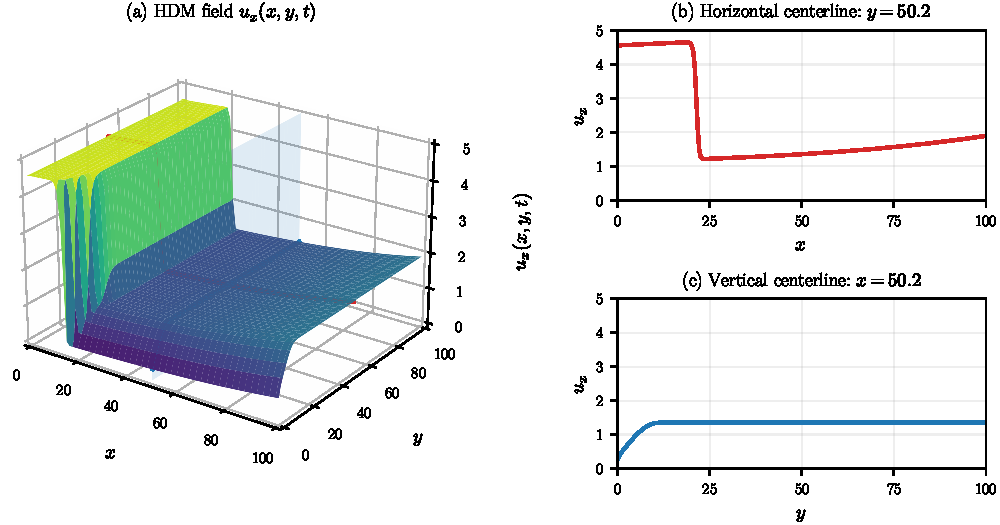
\includegraphics[width=\textwidth]{Figures/euclidean_hprom/burgers_problem_3d.pdf}
\caption{Representative HDM solution of the two-dimensional Burgers problem
at $\mub=(4.560,0.0190)$ and $t=7.50$.  Panel~(a) shows the
streamwise field $u_x(x,y,t)$; panels~(b) and~(c) show the corresponding
centerline cuts $u_x(x,y_{\mathrm{mid}},t)$ and
$u_x(x_{\mathrm{mid}},y,t)$.  The red and blue planes in panel~(a) identify
the locations of the two cuts.}
\label{fig:burgers-problem}
\end{figure}
Nine HDM trajectories on the $3\times3$ grid
$\{4.25,4.875,5.50\}\times\{0.015,0.0225,0.03\}$ define the centered
POD basis.  Its 151 retained modes capture $99.9900\%$ of the snapshot
energy.  This basis and its reference state remain fixed throughout the study.
The upper-left panel of Figure~\ref{fig:parameter-space} shows this
baseline grid together with the validation and reporting locations defined
below.

The learned models are trained on complete coordinates from the
151-coordinate linear HPROM of Section~\ref{sec:linear-hprom}, not on
orthogonal projections of HDM snapshots.  Its positive cubature rule is
constructed from the baseline data and then frozen.  For training parameters
$\{\mub_j\}_{j=1}^{N_\mu}$, the coordinate labels are
\begin{equation}
\mathcal D_N^{\mathrm H}=
\left\{(\mub_j,t^m,\q_N^m(\mub_j)):
 j=1,\ldots,N_\mu,\ m=0,\ldots,N_t\right\}.
\label{eq:hprom-coordinate-training-data}
\end{equation}
Here $\q_N^m$ is the particular linear-HPROM trajectory of
\eqref{eq:linear-hprom-reference-trajectory}.  Cases~1--3 use its primary
and secondary blocks; HPROM--POD--AE, POD--NN--ROM, and POD--DL--ROM use
the complete coordinate vector.  This common source of labels controls
for differences in regression data; the direct maps remain nonintrusive
at deployment.

Two complete linear-HPROM trajectories are held out for regression
checkpoint and adaptive-rule selection:
\begin{equation}
\mub^{\mathrm{val},1}=(4.5625,0.02625),\qquad
\mub^{\mathrm{val},2}=(5.1875,0.01875).
\label{eq:validation-points}
\end{equation}
The reporting parameters are
\begin{equation}
\begin{aligned}
\mub^{(v)}&=(4.875,0.0225),&\mub^{(1)}&=(4.560,0.0190),\\
\mub^{(2)}&=(5.190,0.0260),&\mub^{(3)}&=(4.000,0.0330).
\end{aligned}
\label{eq:evaluation-points}
\end{equation}
The verification point $\mub^{(v)}$ belongs to the nine-point training grid;
$\mub^{(1)}$ and $\mub^{(2)}$ are off-grid but in-domain;
$\mub^{(3)}$ is extrapolatory.  Their errors are evaluated after the ANN
checkpoints and adaptive ECM rule have been selected.

All baseline learned models use the same fixed POD coordinates.
HPROM--ANN Cases~1--3 have $n=10$, and HPROM--POD--AE and POD--DL--ROM have
$n_z=10$.  The parameter--time master map predicts the complete reference
coordinate vector,
\begin{equation}
\mathcal G_q:(\mub,t)\longmapsto\widehat{\q}_N\in\mathbb R^{151},\qquad
\mathcal M(\mub,t)=\bigl[\mathcal G_q(\mub,t)\bigr]_{11:151}.
\label{eq:master-map}
\end{equation}
POD--NN--ROM deploys $\mathcal G_q$ directly; HPROM--ANN Case~2 solves its
first ten coordinates while prescribing the 141-coordinate tail; and
HPROM--ANN Case~2+$\mathbf B_3$ adds three online residual-selected
amplitudes to that same tail prediction.  Thus these three deployments
share a trained network.
HPROM--ANN Cases~1--3 and HPROM--POD--AE use coordinate mean-squared-error
losses with scaling embedded in their networks.  POD--DL--ROM combines
prediction, latent-consistency, and reconstruction losses with weights
$1$, $0.03$, and $0.01$, respectively.
Table~\ref{tab:training} reports baseline architecture sizes and coordinate
regression errors.  The latter concern each map's own output coordinates,
not the reconstructed state error.
In the model-comparison tables, \emph{online size} counts unknowns solved
through the governing residual at each time step; a dash marks a direct
map without a residual solve.
\begin{table}[H]
\centering
\caption{Baseline regression architectures and relative Frobenius errors
(\%) on training and held-out parameter-validation coordinates.
Architectures list hidden-layer widths;
$\mathcal E$ and $\mathcal D$
denote the autoencoder's encoder and decoder, while $\mathcal G_z$ is
the additional parameter--time latent predictor of POD--DL--ROM.
The POD--NN--ROM row repeats the architecture, parameter count, and
full-coordinate regression errors of the master map shared with HPROM--ANN
Case~2; HPROM--ANN Case~2+$\mathbf B_3$ also reuses it.}
\label{tab:training}
\papertable{tables/euclidean_hprom/training_baseline.tex}
\end{table}

Conventional learned HPROMs have separate, map-specific positive ECM rules
constructed as in Section~\ref{sec:nonlinear-ecm}.  Their entity-contribution
matrices use HDM states from the nine baseline parameters fitted onto each
trained trial map, with a $2\%$ parameter--time state sample and a
$10^{-8}$ relative singular-value cutoff.  Their rules retain 901 residual
cells, versus 5621 for the fixed linear-HPROM rule.  The adaptive rule is
described in Section~\ref{sec:hprom-b3-results}.

For a reporting parameter $\mub$, collect all 501 HDM and reduced time states
in $\mathbf U$ and $\widetilde{\mathbf U}^{\mathrm{ROM}}$, respectively.
The online state-history error is
\begin{equation}
e_u(\mub)=100\frac{\norm{\mathbf U-
\widetilde{\mathbf U}^{\mathrm{ROM}}}_F}{\norm{\mathbf U}_F}.
\label{eq:state-error}
\end{equation}
The mean in each table averages only $\mub^{(v)},\mub^{(1)},\mub^{(2)}$;
extrapolation is separate.  The fixed linear HPROM is a reference model,
not an $e_u$ lower bound: LSPG minimizes a discrete residual, not this
HDM-relative state error.

\subsection{Nine-trajectory baseline: accuracy and the Case--2 gap}
\label{sec:hprom-results}
Table~\ref{tab:online-state} gives the baseline online state errors.
The HPROM--ANN Case~2+$\mathbf B_3$ row is included for direct comparison
but is interpreted in Section~\ref{sec:hprom-b3-results}; the present discussion
first examines the conventional models.
\begin{table}[H]
\centering
\caption{State-history errors $e_u$ (\%) at the nine-trajectory budget.
The mean covers the three in-domain parameters; the last column is
extrapolatory.  The horizontal rule separates residual-solving HPROMs from
direct nonintrusive maps.  HPROM--ANN Case~2+$\mathbf B_3$ has online size 13:
ten primary coordinates and three additional solved amplitudes.  The
linear HPROM has online size 151; direct maps have a dash.  The adaptive
row uses a different initial-state
representation, discussed in Section~\ref{sec:hprom-b3-results}.}
\label{tab:online-state}
\papertable{tables/euclidean_hprom/baseline_state.tex}
\end{table}

The linear HPROM has mean state error $0.441\%$.
HPROM--ANN Cases~1 and~3 and HPROM--POD--AE give $0.553\%$, $0.494\%$, and
$0.583\%$, respectively.  HPROM--ANN Case~2 gives $1.620\%$, close to
$1.701\%$ for the direct POD--NN--ROM using the same master network.
Solving the primary coordinates therefore helps only modestly in-domain
when the secondary block remains prescribed.  At the extrapolatory point,
HPROM--ANN Case~2 gives $2.801\%$ versus POD--NN--ROM's $5.102\%$; the sampled
residual does provide a useful correction, but cannot adjust the injected
tail.  Figure~\ref{fig:hprom-baseline-solutions} checks these aggregate
errors against physical solution profiles.
\begin{figure}[H]
\centering
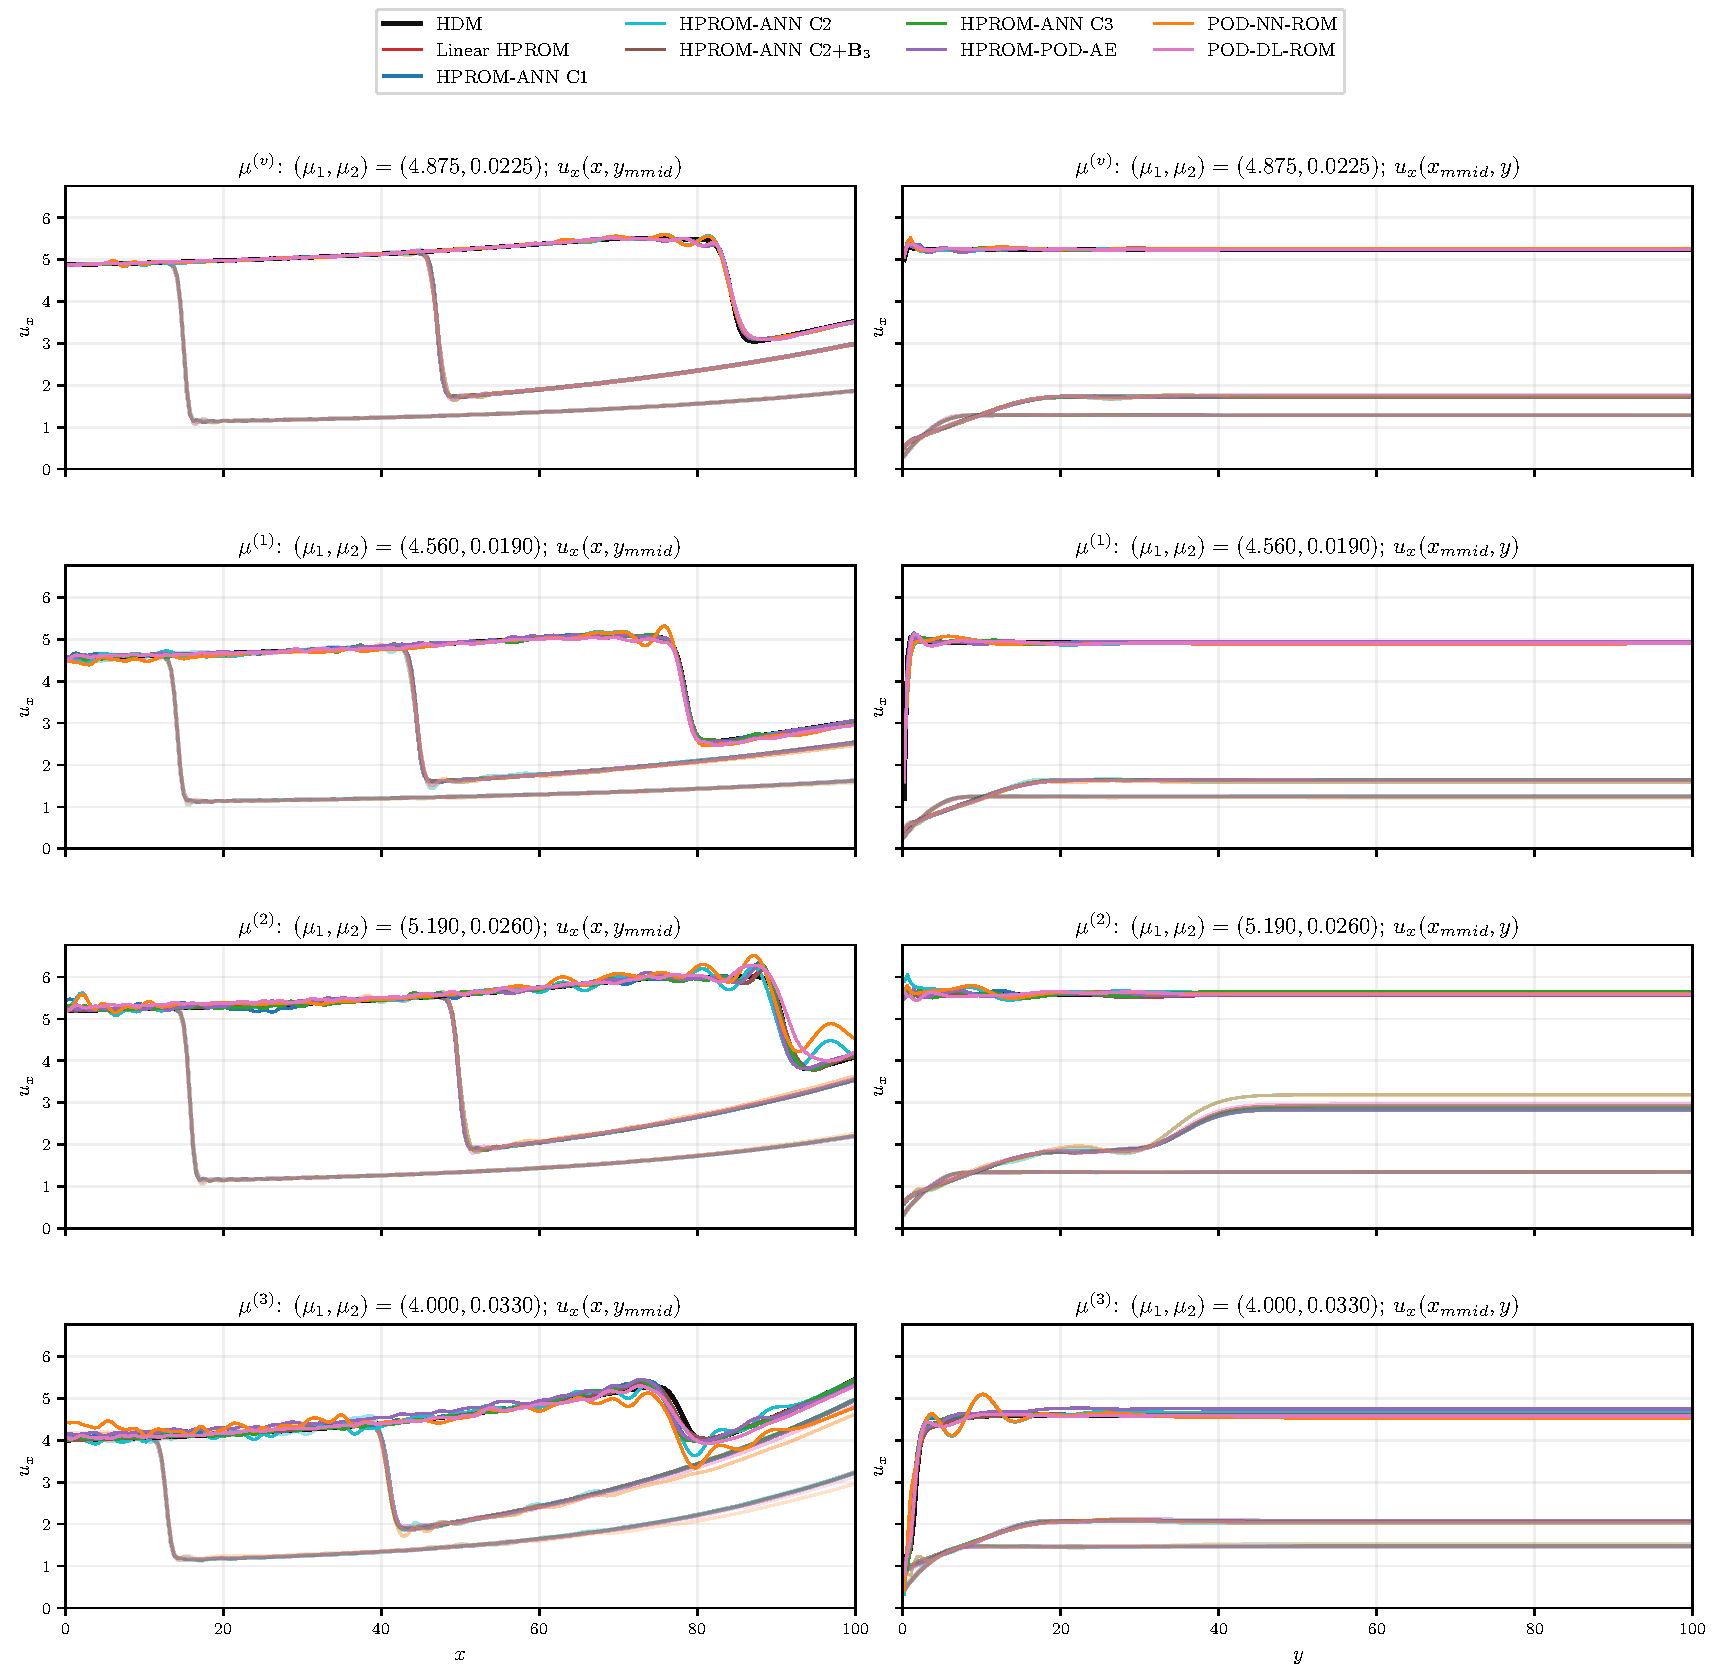
\includegraphics[width=\textwidth,height=.72\textheight,keepaspectratio]{Figures/euclidean_hprom/baseline_solutions.pdf}
\caption{Solution cut-plane overlays for the nine-trajectory training budget
at the four reporting parameters.  Columns show $u_x(x,y_{\mathrm{mid}})$ and
$u_x(x_{\mathrm{mid}},y)$; increasing opacity denotes $t=5,15,25$.
All model curves are solid.  Overlapping profiles should be interpreted
alongside the space--time errors of Table~\ref{tab:online-state}.}
\label{fig:hprom-baseline-solutions}
\end{figure}

The Case--2 gap suggests two distinct responses.  One can improve the
parameter--time map with additional linear-HPROM trajectories, or retain
the nine-trajectory map and allow selected secondary patterns to respond
to the current residual.  We test the latter first because it is the
method developed in Section~\ref{sec:adaptive-case2}; enrichment is
assessed separately in Section~\ref{sec:hprom-enrichment}.

\subsection{Residual-adaptive correction without additional training data}
\label{sec:hprom-b3-results}
HPROM--ANN Case~2+$\mathbf B_3$ uses the same baseline master map as
HPROM--ANN Case~2 and POD--NN--ROM.  Following
Section~\ref{sec:adaptive-positive-rule}, 90 predictor anchors from the
nine baseline parameters yield an 839-cell positive ECM rule, with
relative compression tolerance $0.01$ and ECM integration tolerance
$10^{-8}$.  The rule is selected using the held-out validation parameters
and then fixed for all four reporting points.

The adaptive computation starts from the known initial state represented
in the complete linear space,
\begin{equation}
\qtot^0=\mathbf V_{\mathrm{tot}}^T(\uvec_0-\uvec_{\mathrm{ref}}),\qquad
\utilde_r^0=\uvec_{\mathrm{ref}}+\mathbf V_{\mathrm{tot}}\qtot^0.
\label{eq:adaptive-common-initial}
\end{equation}
Conventional learned HPROMs instead initialize on their trained manifolds.
The main HPROM comparison therefore includes an initialization difference;
the matched-initialization full-residual controls in
Appendix~\ref{sec:adaptive-results} help isolate direction selection.

With $n=10$ and $\bar n=141$, the three columns of
$\mathbf B_3\in\mathbb R^{141\times3}$ represent patterns over the entire
secondary block, not just coordinates 11--13.  All three directions were
attained throughout the 500-step reporting trajectories.  The corrected
HPROM has $0.454\%$ mean and $0.844\%$ extrapolatory state error, near the
$0.441\%$ and $0.850\%$ of the fixed linear HPROM.

In the matched-initialization full-residual PROM control of
Appendix~\ref{sec:adaptive-results}, the three-direction correction gives
$0.447\%$ mean state error at 13 unknowns, versus $1.513\%$ when the next
three POD coordinates are solved instead.  This supports the importance
of direction selection in that separate setting.
Figure~\ref{fig:hprom-b3-histories} resolves the baseline HPROM errors in
time.
\begin{figure}[H]
\centering
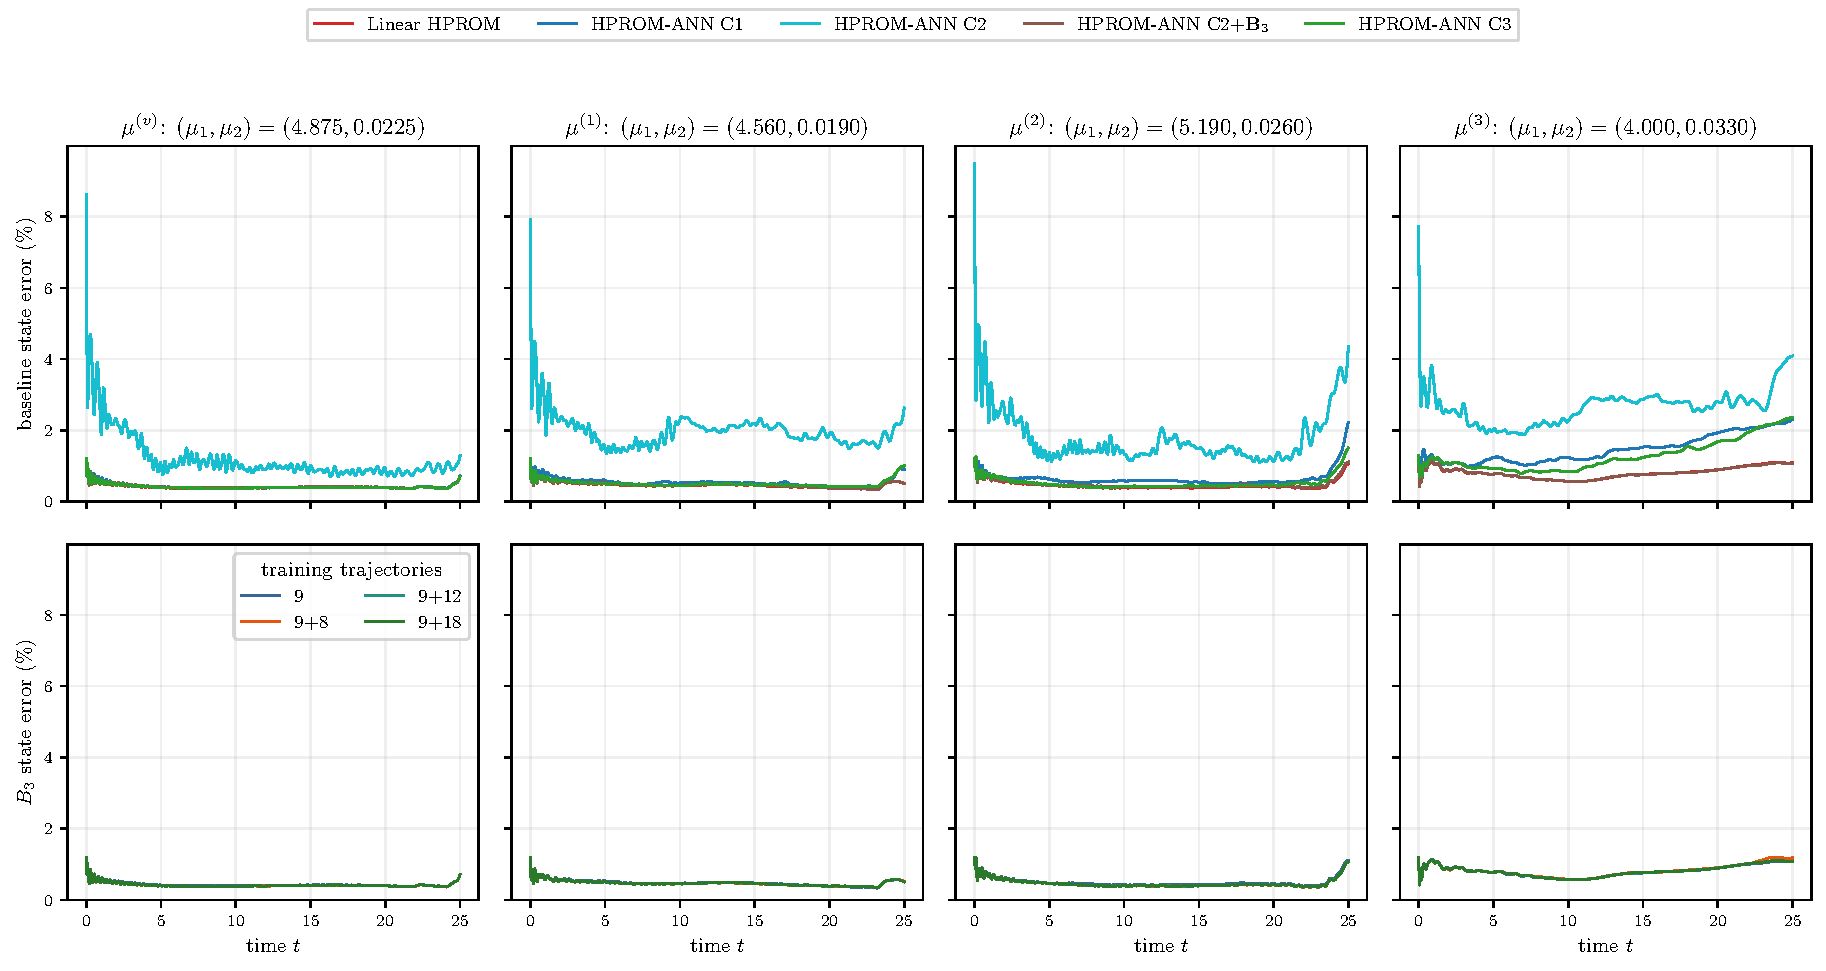
\includegraphics[width=\textwidth]{Figures/euclidean_hprom/b3_histories.pdf}
\caption{Instantaneous HDM-relative state errors for the linear HPROM,
HPROM--ANN Cases~1--3, and HPROM--ANN Case~2+$\mathbf B_3$ at the four reporting parameters.
Panels share logarithmic ordinate limits; all plotted errors are positive.
Instantaneous ratios differ from the
space--time Frobenius errors in Table~\ref{tab:online-state}.}
\label{fig:hprom-b3-histories}
\end{figure}

Table~\ref{tab:hprom-timing} compares baseline state accuracy and mean
wall-clock time over the three in-domain reporting parameters.  Speedup
is the ratio of mean HDM time to mean model time.  The table's element
count is the full mesh for the HDM and the selected ECM support for each
HPROM.

The number of residual-solved unknowns is $N=125{,}000$ for the HDM,
$n_{\mathrm{tot}}=151$ for the linear HPROM, $n_z=10$ for HPROM--POD--AE,
and $n=10$ for HPROM--ANN Cases~1--3.  HPROM--ANN Case~2+$\mathbf B_3$
instead solves $n+r=13$ unknowns while retaining $n=10$ and $\bar n=141$.
\begin{table}[H]
\centering
\caption{Baseline in-domain state accuracy, wall-clock time, and HDM-relative
speedup for the two-dimensional parametric Burgers problem.  The HDM and
linear-HPROM timings use 24 numerical threads; all other timings use one.
Direct-map times and factors marked $^\dagger$ cover coefficient-history
inference only (ten repeats), excluding full-state reconstruction.}
\label{tab:hprom-timing}
\papertable{tables/euclidean_hprom/timing_baseline.tex}
\end{table}
At the nine-trajectory budget, HPROM--ANN Case~2+$\mathbf B_3$ gives the
strongest measured accuracy--time balance among learned residual-solving
HPROMs: it is both faster and more accurate than Cases~1 and~3 and
HPROM--POD--AE, including a $3.5\times$ speedup over Case~1.  It is
$12.5\times$ faster than the linear HPROM at nearly the same mean state
error.  Uncorrected Case~2 is only slightly faster but has $1.620\%$
mean error instead of $0.454\%$.

\subsection{Enriching the learned maps with linear-HPROM trajectories}
\label{sec:hprom-enrichment}
Once the linear HPROM has been built, it can supply further complete-coordinate
trajectories for training the learned maps at a lower solve cost than the
HDM; its measured wall time is about one tenth of the HDM's in
Table~\ref{tab:hprom-timing}.  Enriching these regression data is therefore
a practical way to improve the closures and direct predictors without
enlarging the fixed POD basis.  For intrusive models, the learned trial
maps still constrain what the residual solve can represent; for direct
models, the learned map supplies the full coordinate prediction.  We
therefore test enrichment for all conventional learned families, not only
Case~2.

A nested Latin-hypercube design adds equal numbers of interior and margin
parameters to the original nine-point grid.  The four budgets are $9$,
$9+8$, $9+12$, and $9+18$ trajectories.  Margin points lie in the four
strips between the original parameter box and a rectangle enlarged by
$25\%$ on each side.
Figure~\ref{fig:parameter-space} shows the resulting sampling geometry,
including the reporting points.
\begin{figure}[H]
\centering
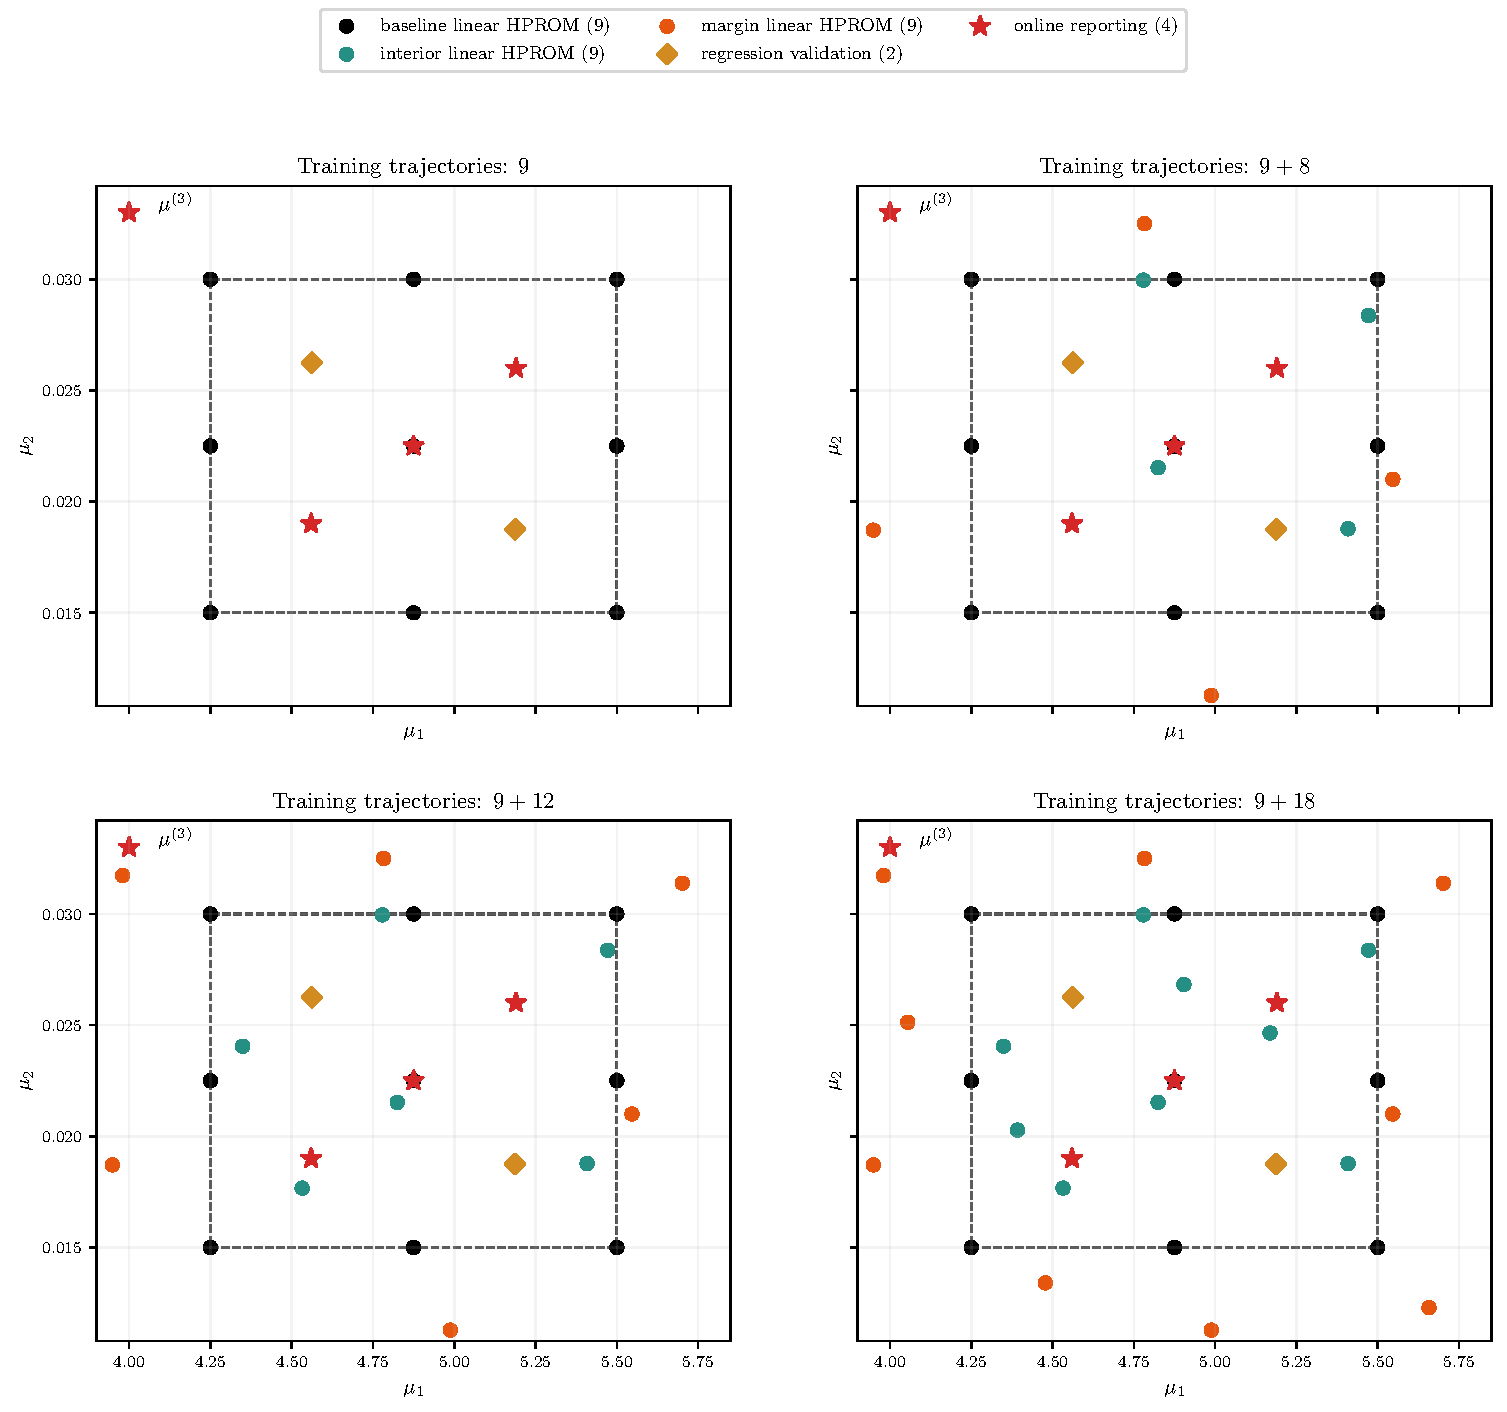
\includegraphics[width=\textwidth]{Figures/euclidean_hprom/sampling.pdf}
\caption{Nested linear-HPROM coefficient-data layouts: baseline, $9+8$,
$9+12$, and $9+18$.  Black circles are baseline parameters; coloured
points are added interior and margin parameters; diamonds are held-out
regression-validation parameters; stars are reporting parameters.
The original parameter box is outlined.}
\label{fig:parameter-space}
\end{figure}

Each family is retrained at each budget with the same architecture, nominal
loss, and checkpoint-selection parameters.  Conventional intrusive models
receive a new map-specific positive ECM rule; the linear-HPROM reference
and its rule remain fixed.  The results thus assess the full enriched
workflow, with both a retrained map and a rebuilt ECM rule where applicable.
The baseline HPROM--ANN Case~2+$\mathbf B_3$ is already near the fixed
linear-HPROM accuracy level (Table~\ref{tab:online-state}).  Here we ask
how far additional data take the \emph{conventional} models toward that
level; the adaptive model remains at its nine-trajectory baseline.
Combining it with an enriched map would require a new adaptive ECM rule
and is not part of this comparison.

Table~\ref{tab:hprom-enrichment-state} and
Fig.~\ref{fig:hprom-enrichment-state} give the online state-error response.
Appendix~\ref{app:hprom-details} gives the pointwise values behind the
in-domain means.
\begin{table}[H]
\centering
\caption{State-history errors $e_u$ (\%) at the nested data budgets.
Each budget gives the in-domain mean and extrapolation; the linear HPROM
is fixed: ``unchanged'' denotes its baseline errors, not a distinct
enriched model.  HPROM--ANN Case~2+$\mathbf B_3$ uses the nine-trajectory
master map; dashes mark budgets without an adaptive result.
The horizontal rule separates intrusive HPROMs from
nonintrusive direct maps.  Online size has the same meaning as in
Table~\ref{tab:online-state}.}
\label{tab:hprom-enrichment-state}
\papertable{tables/euclidean_hprom/enrichment_state.tex}
\end{table}
\begin{figure}[H]
\centering
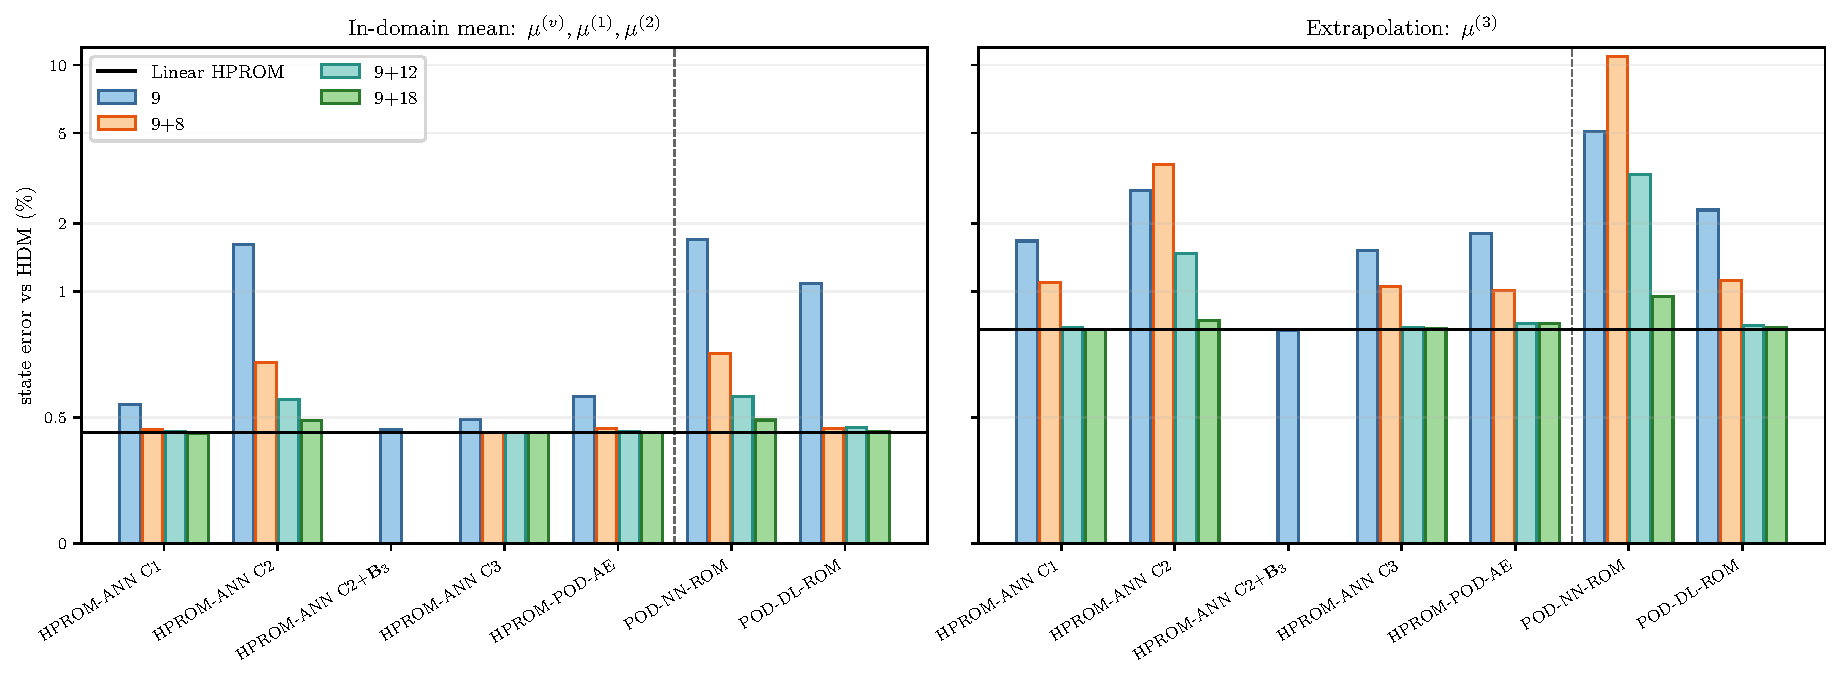
\includegraphics[width=\textwidth]{Figures/euclidean_hprom/enrichment_state.pdf}
\caption{Enrichment response of the conventional model families.
Left: in-domain mean; right: extrapolation.  Both panels share the same
ordinate, linear below $1\%$ and logarithmic above.  Black horizontal lines
mark the frozen linear HPROM; dashed vertical lines separate residual-solving
from direct models.
The single blue bar between Cases~2 and~3 marks the
Case~2+$\mathbf B_3$ result at the baseline budget
(Table~\ref{tab:hprom-enrichment-state}).}
\label{fig:hprom-enrichment-state}
\end{figure}

Enrichment improves the in-domain mean of every conventional learned
family between the nine-trajectory baseline and $9+18$ (Table~\ref{tab:hprom-enrichment-state}).
HPROM--ANN Case~2 falls from $1.620\%$ to $0.488\%$, and POD--NN--ROM,
which shares its master map, falls from $1.701\%$ to $0.490\%$.
HPROM--ANN Cases~1 and~3, HPROM--POD--AE, and POD--DL--ROM also improve,
ending between $0.438\%$ and $0.445\%$ in-domain.  The shared map's
held-out coordinate error falls from $4.402\%$ to $1.006\%$
(Appendix~\ref{app:hprom-details}).  The enriched workflow benefits even
models that were already close to the $0.441\%$ linear-HPROM reference.

The comparison also shows what the residual-adaptive correction buys at
the original data budget.  With nine training trajectories,
HPROM--ANN Case~2+$\mathbf B_3$ gives $0.454\%$ in-domain mean error and
$0.844\%$ at extrapolation.  Conventional Case~2 approaches these values
only at $9+18$, where it gives $0.488\%$ and $0.886\%$.  These are
comparisons of deployed methods, including their different initialization
and ECM rules.

Extrapolation does not follow the same smooth trend: the first enrichment
worsens Case~2 and POD--NN--ROM at $\mub^{(3)}$ before later budgets improve
them.  The nested design changes how closely the added points cover this
extrapolatory location (Fig.~\ref{fig:parameter-space}); the maps and ECM
rules also change.  Thus the number of new trajectories alone does not
predict accuracy at a particular point outside the training box.

Thus enrichment is a valuable offline strategy for the learned models
tested here.  Residual adaptation addresses a different weakness:
it lets Case~2 correct its prescribed secondary tail online even when the
regression map is trained on only nine trajectories.

\section{Conclusions}
\label{sec:conclusions}
Using a common POD basis and linear-HPROM training trajectories, this
study systematically compares intrusive HPROM--ANN and HPROM--POD--AE
models with nonintrusive POD--NN--ROM and POD--DL--ROM predictors.
The parameter--time closure of HPROM--ANN Case~2 has a simple online
tangent, but its prescribed secondary coordinates cannot respond to the
current residual.  The residual-adaptive extension developed here restores
that response through a small secondary Krylov space, rebuilt at each time
step and held fixed during its nonlinear solve.

With nine training trajectories on the Burgers benchmark, three adaptive
directions reduce Case~2's mean in-domain state error from $1.620\%$ to
$0.454\%$ using 13 online unknowns, near the $0.441\%$ error of the
151-coordinate linear HPROM.  Under the measured timing protocol, this is
the strongest accuracy--time balance among learned residual-solving
HPROMs: $122\times$ faster than the HDM, $12.5\times$ faster than the
linear HPROM, and $3.5\times$ faster and more accurate than HPROM--ANN
Case~1.  A separate equal-dimensional full-residual control shows that
direction selection, not only the three extra unknowns, drives the
recovery.  Its rank diagnostic gives further coordinate-error reduction
beyond $r=3$ but little additional reduction in the converged residual;
three directions are already effective for the reported HPROM.

The study also illustrates a multifidelity reduced-order training workflow:
HDM trajectories establish the POD basis, while a lower-cost linear HPROM
supplies further coordinate histories to train both intrusive nonlinear
trial maps and nonintrusive coefficient predictors.  Across the tested
budgets, this enrichment brings every conventional learned model toward
the fixed linear-HPROM accuracy level in-domain, and direct maps become
competitive there.  The distinction is clearest with sparse data at the
extrapolatory point $\mub^{(3)}$: POD--NN--ROM and intrusive HPROM--ANN
Case~2 share a network yet give $5.102\%$ and $2.801\%$ state error,
respectively, while Case~2+$\mathbf B_3$ reaches $0.844\%$.  Residual-based
online correction can thus mitigate errors beyond the sampled parameter
region, whereas a direct map relies on its learned extrapolation.  This
capability is especially relevant to demanding engineering simulations.
Extending these complementary strategies to more challenging
industrial-scale problems is a natural next step.

\appendix
\section{Full-Residual PROM Direction-Selection Controls}
\label{sec:adaptive-results}
\subsection{Diagnostic protocol}
\label{sec:adaptive-protocol}
These previously completed experiments use full-residual PROM trajectories
and a master ANN trained on nine linear-PROM trajectories, with the two
validation parameters in \eqref{eq:validation-points}.  They are not HPROM
runs, do not use the HPROM-trained master network, and report no timings.
Their purpose is to isolate trial-space orientation before cubature.
In this appendix and Appendix~\ref{sec:prom-results}, $\q_N$ denotes
the corresponding full-residual linear-PROM trajectory from
\eqref{eq:linear-prom}, and $\mathbf Q_N$ its complete coordinate history.
For the rank diagnostic alone, let $\mathbf Q_{\mathrm{tot}}^{\mathrm{ROM}}$
be the compared complete coordinate history and define
\begin{equation}
e_q(\mub)=100\frac{\norm{\mathbf Q_N-
\mathbf Q_{\mathrm{tot}}^{\mathrm{ROM}}}_F}{\norm{\mathbf Q_N}_F}.
\label{eq:coefficient-error}
\end{equation}
This measures agreement with the linear PROM, not state accuracy against
the HDM.  It is used only to diagnose the direction-selection mechanism;
the state comparisons below use $e_u$ from \eqref{eq:state-error}.
All compared trajectories use the known initial representation
\eqref{eq:adaptive-common-initial}, the same full residual, and the same
nominal nonlinear solver settings.  The tested ranks are
\begin{equation}
r\in\{0,1,2,3,5,10\}.
\label{eq:adaptive-tested-ranks}
\end{equation}
The $n=10$ adaptive model is paired at every rank with conventional Case~2
solving $10+r$ primary coordinates and using the trial map
\begin{equation}
\utilde_{n+r}^{\mathrm{C2}}(\mathbf x;\mub,t)
=\uvec_{\mathrm{ref}}+\mathbf V_{1:n+r}\mathbf x+
\mathbf V_{n+r+1:151}
\bigl[\mathcal G_q^{\mathrm{PROM}}(\mub,t)\bigr]_{n+r+1:151},
\qquad\mathbf x\in\mathbb R^{n+r}.
\label{eq:case2-equal-dimension-control}
\end{equation}
Thus each pair has the same number of unknowns and the same network.
The choice $r=3$ was frozen by preliminary screening at the two validation
parameters before reporting-point evaluation.  The subsequent
validation-only sweep over $r\in\{0,1,2,3,5,10\}$ documents rank
dependence without reselecting that choice.  These parameters also serve
network validation, so the sweep is diagnostic rather than an independent
generalization test.  Every run uses the same master ANN,
$n=10$, the complete residual and Jacobian, and the common initial
representation \eqref{eq:adaptive-common-initial}.  Thus $r=0$ is the
matched uncorrected Case~2 trajectory.  For every $r$, the comparison also
includes the plain Case--2 map \eqref{eq:case2-equal-dimension-control} with
$n=10+r$.  In particular, $\mathbf B_5$ and $\mathbf B_{10}$ are compared
with Case~2 at $n=15$ and $n=20$, respectively.
Figure~\ref{fig:adaptive-rank-validation} compares the resulting
equal-size trajectories through $e_q$ and the converged-residual reduction.

\begin{figure}[H]
\centering
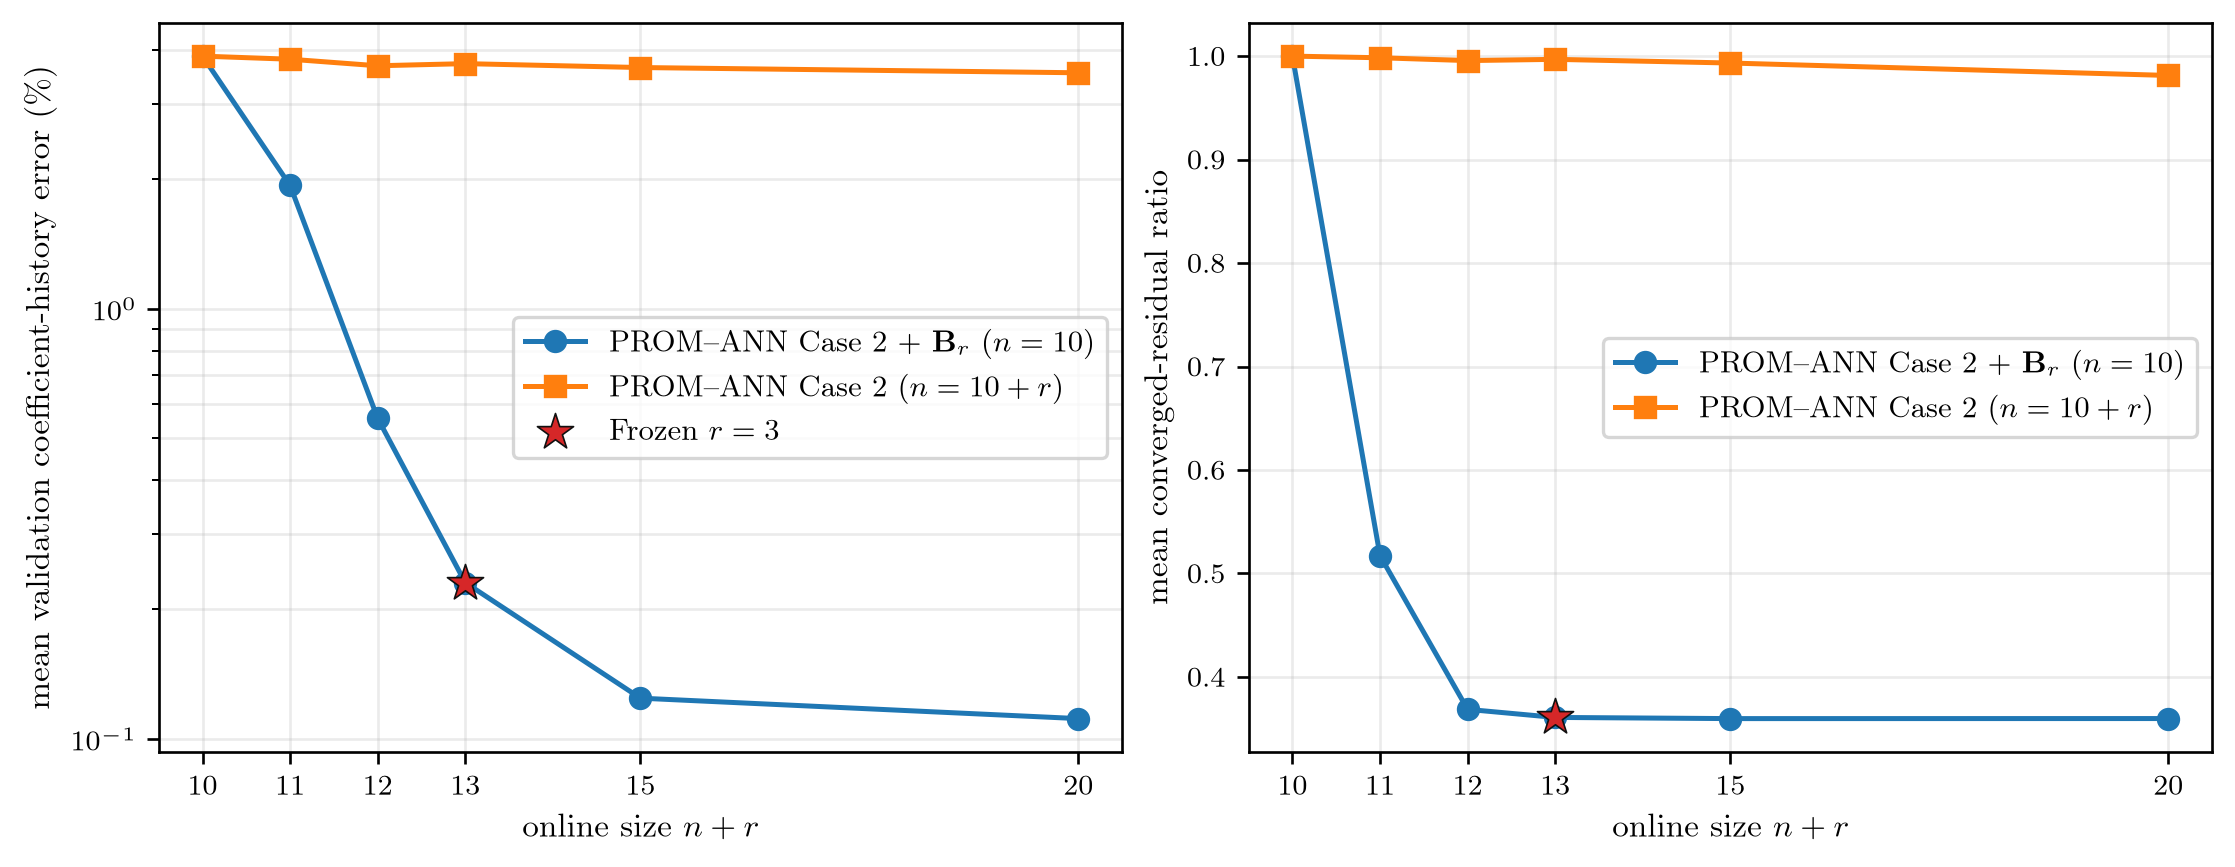
\includegraphics[width=0.94\textwidth]{Figures/euclidean_prom_only/euclidean_case2_rank_validation.png}
\caption{Validation-only comparison at equal online size $10+r$.
Left: mean complete coefficient-history error against linear PROM.
Right: residual norm at termination of each nonlinear solve, averaged over
time steps and the two validation parameters, then normalized by the common
$r=0$, $n=10$ value.  The $e_q$ panel diagnoses agreement with a PROM
reference, not HDM-relative state accuracy.  The star identifies the
previously frozen $r=3$ rather than a rank selected from this expanded
sweep.}
\label{fig:adaptive-rank-validation}
\end{figure}

In this diagnostic, $e_q$ decreases with corrected rank while remaining
nearly unchanged for ordinary Case~2 at equal online size.  At 13 unknowns,
for example, the two mean validation errors are $0.231\%$ and $3.720\%$.

The residual data give the same qualitative distinction.  The adaptive
mean converged-residual ratio decreases from one to $0.361$ by $r=3$ and
then remains essentially unchanged.  The corresponding conventional ratio
remains above $0.982$ even at $n=20$.  Therefore the observed improvement
cannot be explained by online dimension alone.  For this benchmark, the
Krylov directions in \eqref{eq:adaptive-krylov} capture combinations of the
secondary coordinates that are much more effective for the local LSPG
problem than the next POD modes selected by snapshot energy.

This comparison remains diagnostic rather than an error theorem.  The
nested-space result \eqref{eq:adaptive-nested-bound} concerns a fixed
linearization, whereas Fig.~\ref{fig:adaptive-rank-validation} reports
complete nonlinear trajectories.
Moreover, the two parameters used here also served for network validation.
The expanded sweep therefore documents rank dependence and the mechanism of
the recovery, but it neither supplies an independent generalization estimate
nor changes the previously frozen reporting choice $r=3$.  Consequently,
only $\mathbf B_3$ and its $n=13$ equal-dimensional control are evaluated at
the four reporting parameters below.

\subsection{Equal-dimensional control and state accuracy}
We now assess the residual-adaptive construction of
Section~\ref{sec:adaptive-case2} under the dedicated protocol of
Appendix~\ref{sec:adaptive-protocol}.  The notation ``Case~2 + $\mathbf B_3$''
denotes three directions rebuilt at every time step, not a fixed offline
basis.  All learned models in this full-residual comparison retain their
baseline training data.  Section~\ref{sec:hprom-enrichment} separately
examines enriched conventional HPROMs.

\begin{table}[H]
\centering
\caption{Common-initialization full-residual comparison: state-history error
$e_u$ (\%).  Every learned model uses baseline training data.  The mean
averages the three in-domain points; the final column is extrapolatory.
Online size counts residual-solved unknowns.  The PROM--ANN Case~2 row
with online size 13 uses 13 primary coordinates and controls for
PROM--ANN Case~2+$\mathbf B_3$ with
$n=10$ and $r=3$, also of online size 13.
The linear PROM is the 151-coordinate reference.}
\label{tab:adaptive-state}
\papertable{tables/euclidean_prom_only/euclidean_case2_adaptive_state.tex}
\end{table}

Table~\ref{tab:adaptive-state} shows a reduction of the mean in-domain state
error from $1.617\%$ for uncorrected Case~2 to $0.447\%$ for the adaptive
variant, a $72.4\%$ reduction.  The latter is close to the linear-PROM
mean of $0.441\%$.  At the extrapolatory parameter the error decreases
from $2.643\%$ to $0.850\%$, also close to the linear reference.
These changes require neither new coefficient training data nor additional
network fitting.  They result from allowing three residual-selected
secondary patterns to be corrected together with the ten primary coordinates.

Merely increasing the primary dimension from $n=10$ to $n=13$ reduces the
mean state error only from $1.617\%$ to $1.513\%$, and the extrapolatory
error from $2.643\%$ to $2.409\%$.  With the same 13 online unknowns,
Case~2+$\mathbf B_3$ gives $0.447\%$ and $0.850\%$, respectively.  The
observed recovery therefore cannot be attributed solely to adding three
degrees of freedom: the residual-selected combinations of the 141 secondary
coordinates are substantially more effective here than freeing POD
coordinates 11--13.

PROM--ANN Case~2+$\mathbf B_3$ improves on PROM--ANN Cases~1 and~3 in mean error and at
extrapolation, but not at every parameter:
Case~3 has a slightly smaller state error at verification.  Likewise, the
linear PROM is not a strict HDM-error lower bound; at $\mub^{(1)}$ the
corrected trajectory has a slightly smaller HDM error than that reference.
Figure~\ref{fig:adaptive-state-histories} shows how the corresponding
instantaneous errors evolve over time at each reporting parameter.

\begin{figure}[H]
\centering
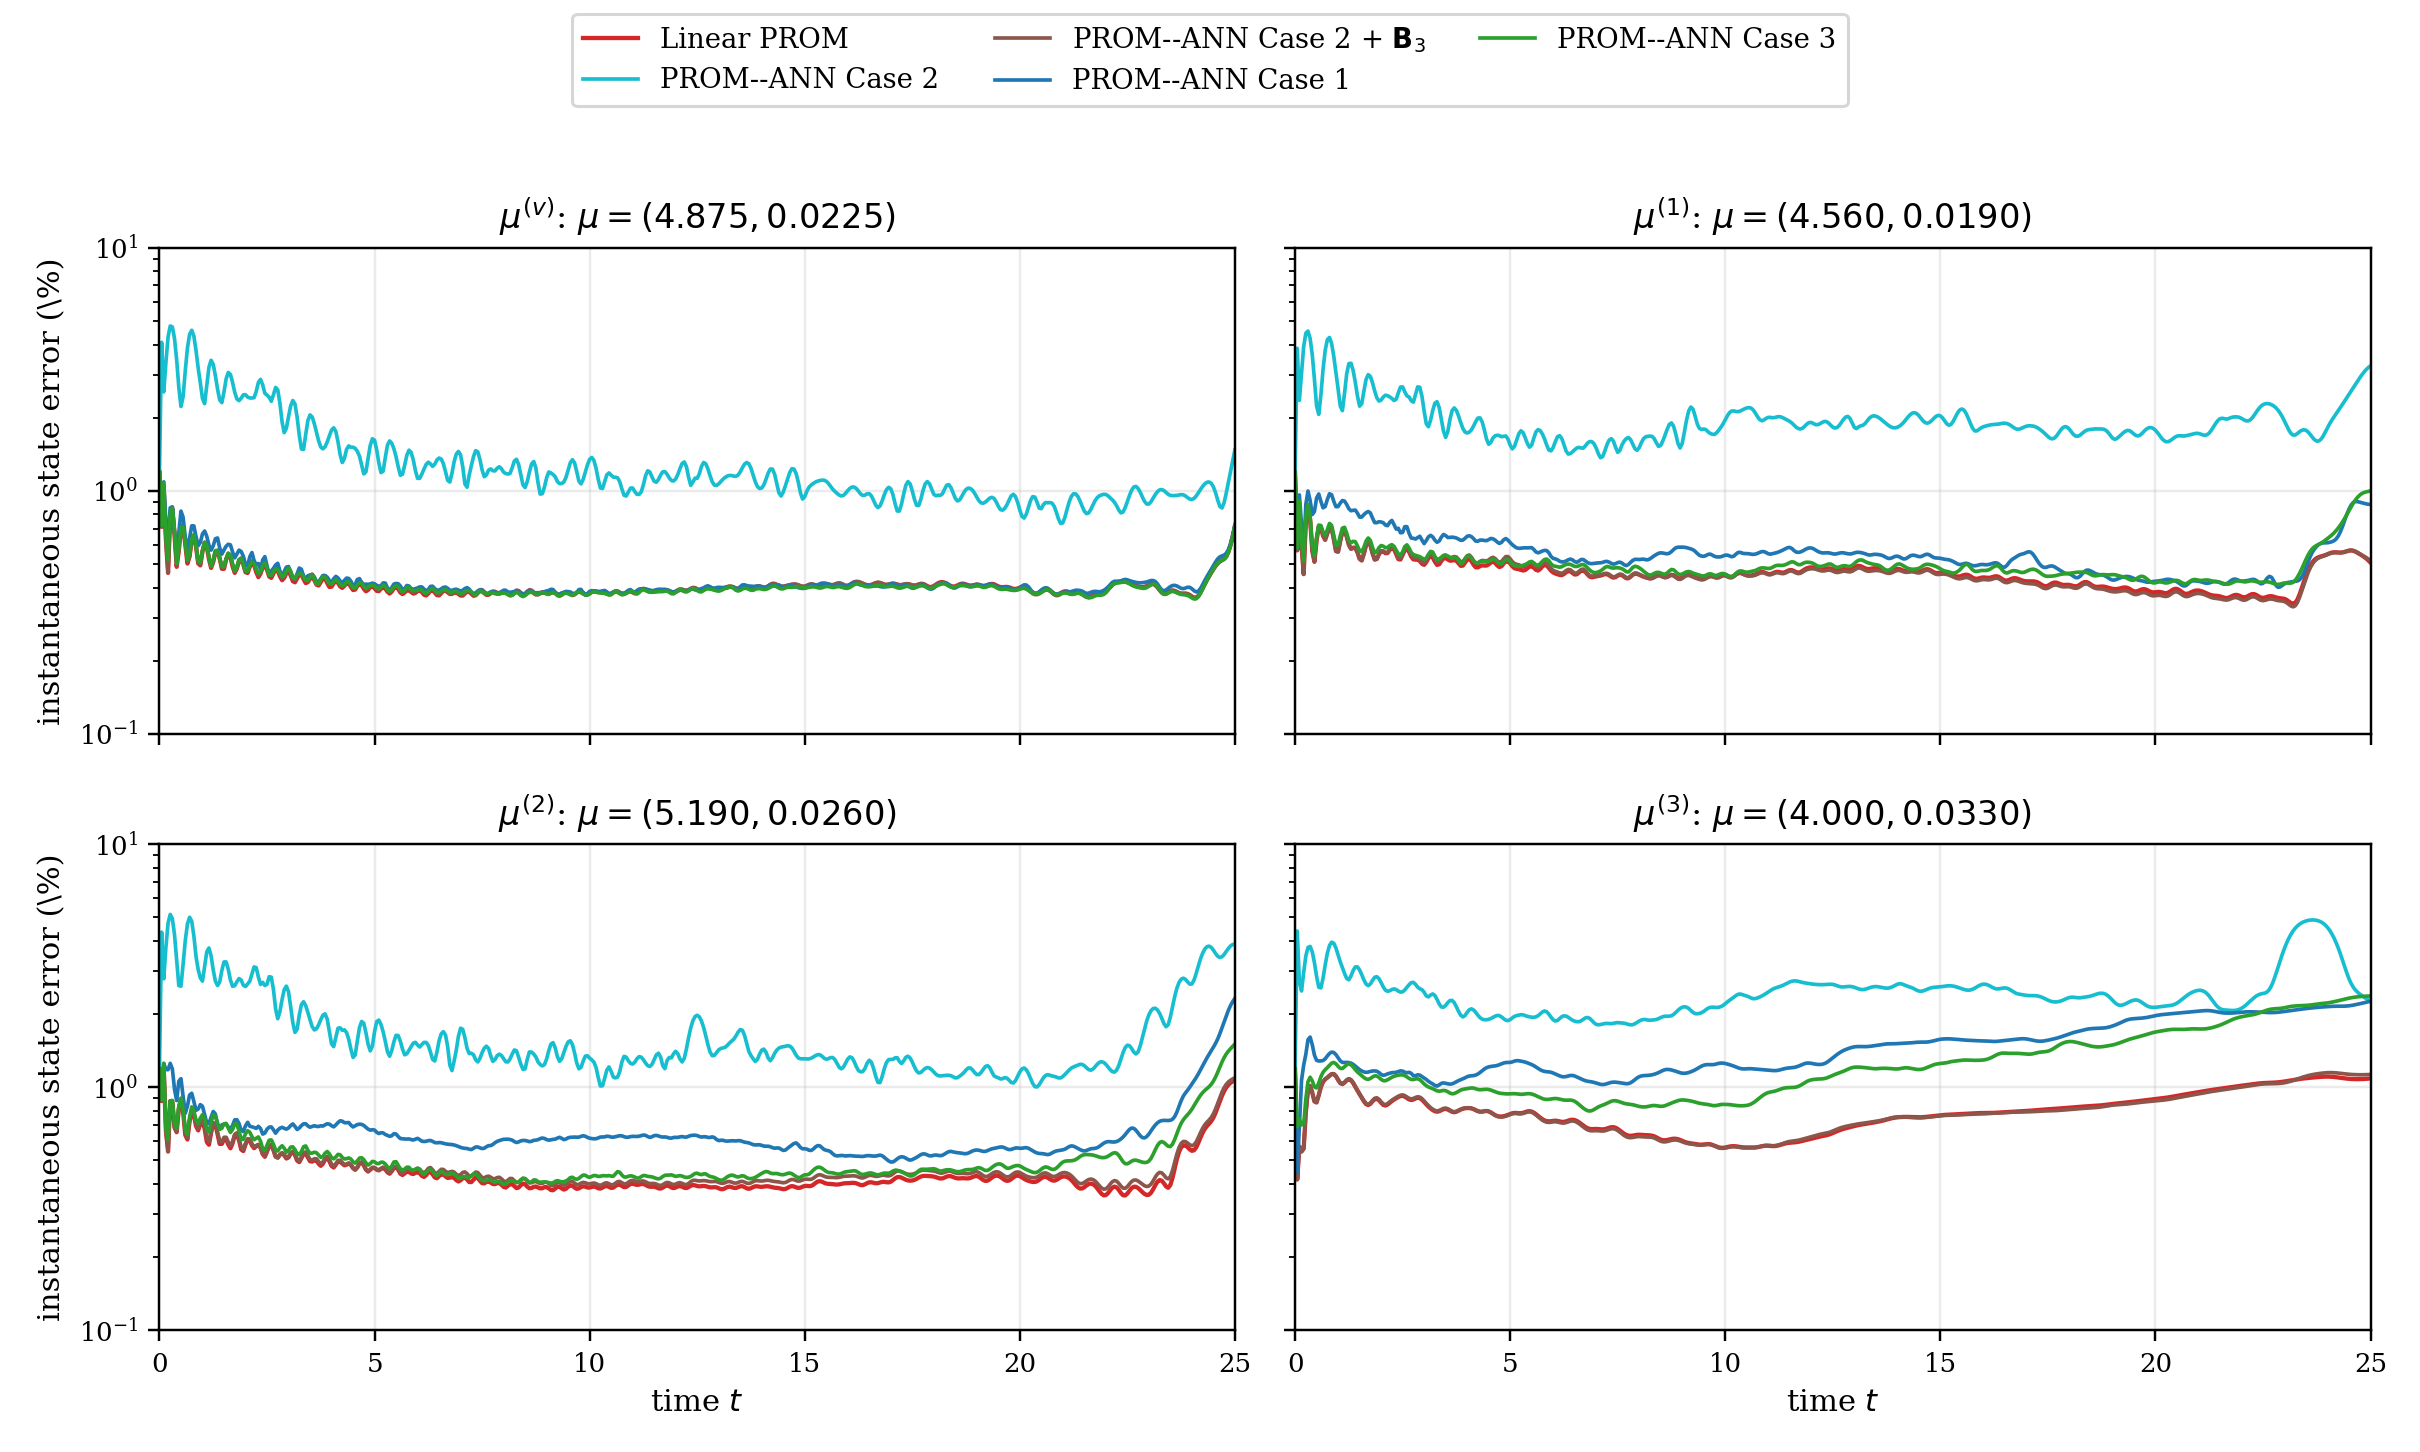
\includegraphics[width=0.96\textwidth]{Figures/euclidean_prom_only/euclidean_case2_adaptive_state_histories.png}
\caption{Instantaneous relative state errors
$100\norm{\uvec(t)-\utilde_{\mathrm{ROM}}(t)}_2/
\norm{\uvec(t)}_2$ for the common-initialization comparison.
Panels follow the four reporting parameters and share logarithmic ordinate
limits; all plotted errors are positive and all model curves are solid.
These time-resolved errors complement, rather than replace, the space--time
norm in Table~\ref{tab:adaptive-state}.}
\label{fig:adaptive-state-histories}
\end{figure}

For these four parameters, a small online secondary correction substantially
closes the baseline Case--2 accuracy gap without enriching its training set.
This is not evidence that enrichment is unnecessary: enrichment changes the
offline data, whereas the adaptive construction uses the current residual
and Jacobian during deployment.  The combination of
Case~2+$\mathbf B_3$ with enriched HPROM training data is not evaluated in
Section~\ref{sec:hprom-enrichment}.
No general state-error guarantee follows from this experiment.

\section{Full-Residual Case--2 Sweep and Perturbation Diagnostic}
\label{sec:prom-results}
The following retained PROM diagnostics motivate secondary correction but
are not evidence about an HPROM perturbation or primary-dimension sweep.
They use the common basis, full-residual linear-PROM references, and
PROM-trained master map of the original campaign.  Their numbers are kept
separate from the linear-HPROM reference used in the main text.  These
retained diagnostic runs also differ from the matched reporting protocol
of Appendix~\ref{sec:adaptive-results}; their Case--2 errors should not
be identified with the rows of Table~\ref{tab:adaptive-state}.

\subsection{Case--2 solved-dimension sweep}
\label{sec:case2-sweep}
The shared master map permits an interpolation between a direct parameter--time
regression and the full-coordinate linear PROM.  Table~\ref{tab:case2-sweep}
and Fig.~\ref{fig:case2-sweep-state} show that increasing $n$ reduces state
error, with the sharpest improvement between $n=50$ and
$n=100$.  This records the balance in this controlled Case--2 setting between
coordinates supplied by the ANN and coordinates corrected by the residual.

\begin{table}[H]
\centering
\caption{Case--2 state errors as the number of residual-solved primary
coordinates is varied.  Entries are HDM-relative state-history errors (\%).
Online size equals $n$ for the Case--2 rows;
the remaining $151-n$ coordinates are prescribed.  The $n=0$ endpoint
is POD--NN--ROM, marked with a dash because it performs no residual solve;
at $n=151$, the model is the full-coordinate linear PROM.  The horizontal
rule separates residual-solving models from the direct map.}
\label{tab:case2-sweep}
\papertable{tables/euclidean_prom_only/euclidean_prom_case2_n_sweep_state_errors.tex}
\end{table}

\begin{figure}[H]
\centering
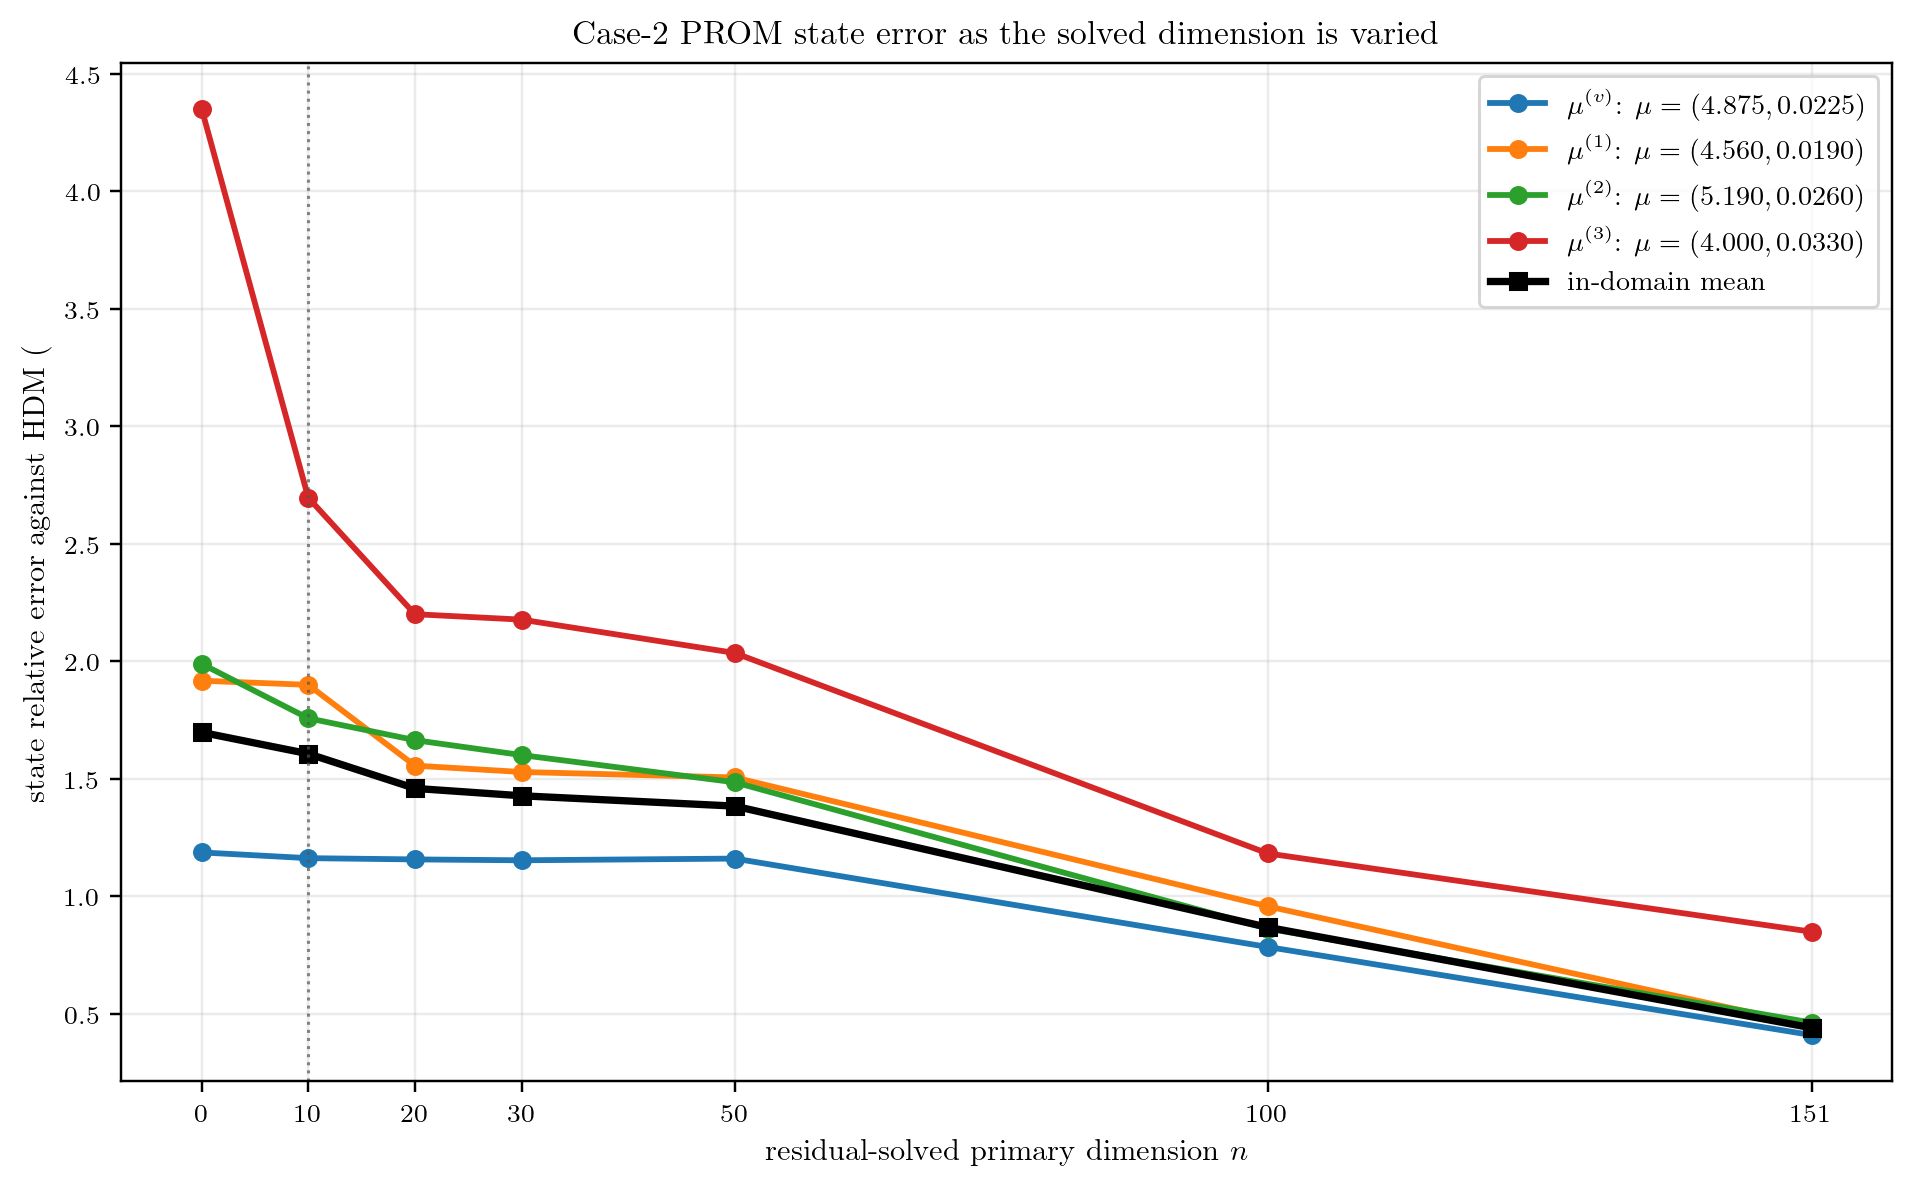
\includegraphics[width=0.78\textwidth]{Figures/euclidean_prom_only/euclidean_prom_case2_n_sweep_state_errors.png}
\caption{Case--2 state error versus the solved primary dimension.  The black
curve is the in-domain mean and the dotted line marks the baseline $n=10$
split.}
\label{fig:case2-sweep-state}
\end{figure}

\subsection{Controlled Case--2 tail perturbation}
\label{sec:tail-perturbation}
To test the transfer mechanism independently of a regression magnitude,
let $\overline{\mathbf Q}_N$ be the last 141 rows of the linear-PROM
coordinate history $\mathbf Q_N$ at a
reporting parameter.  Let
$\widehat{\overline{\mathbf Q}}_N$ collect the corresponding
secondary predictions of the PROM-trained master map.
When their difference is nonzero, prescribe the perturbed history
\begin{equation}
\overline{\mathbf Q}_{\epsilon}
=\overline{\mathbf Q}_N
+\frac{\epsilon}{100}
\frac{\widehat{\overline{\mathbf Q}}_N
-\overline{\mathbf Q}_N}
{\norm{\widehat{\overline{\mathbf Q}}_N
-\overline{\mathbf Q}_N}_F}
\norm{\overline{\mathbf Q}_N}_F.
\label{eq:tail-perturbation}
\end{equation}
The imposed relative secondary-history error is therefore exactly
$\epsilon\%$.  At each time step, Case~2 injects the corresponding column
of $\overline{\mathbf Q}_{\epsilon}$ and solves only the first ten
coordinates.  Thus the diagnostic uses the observed ANN-error
direction but does not conflate its effect with a change of learned model.
Table~\ref{tab:tail-perturbation} and Fig.~\ref{fig:tail-perturbation} show a
monotone transfer from secondary-tail error to the recovered primary block.
The amount of transfer is parameter dependent, so a tail loss alone does not
imply a pointwise primary-coordinate bound.

\clearpage
\begin{table}[H]
\centering
\caption{Primary-coordinate error induced by a controlled secondary-tail
perturbation in Case~2 with $n=10$ (\%).  Each entry is relative to the
corresponding linear-PROM primary history.  The split is fixed at
$n=10$, $\bar n=141$, and online size 10 throughout, so only the imposed
tail error varies by row.}
\label{tab:tail-perturbation}
\papertable{tables/euclidean_prom_only/euclidean_prom_case2_tail_primary_errors.tex}
\end{table}

\begin{figure}[H]
\centering
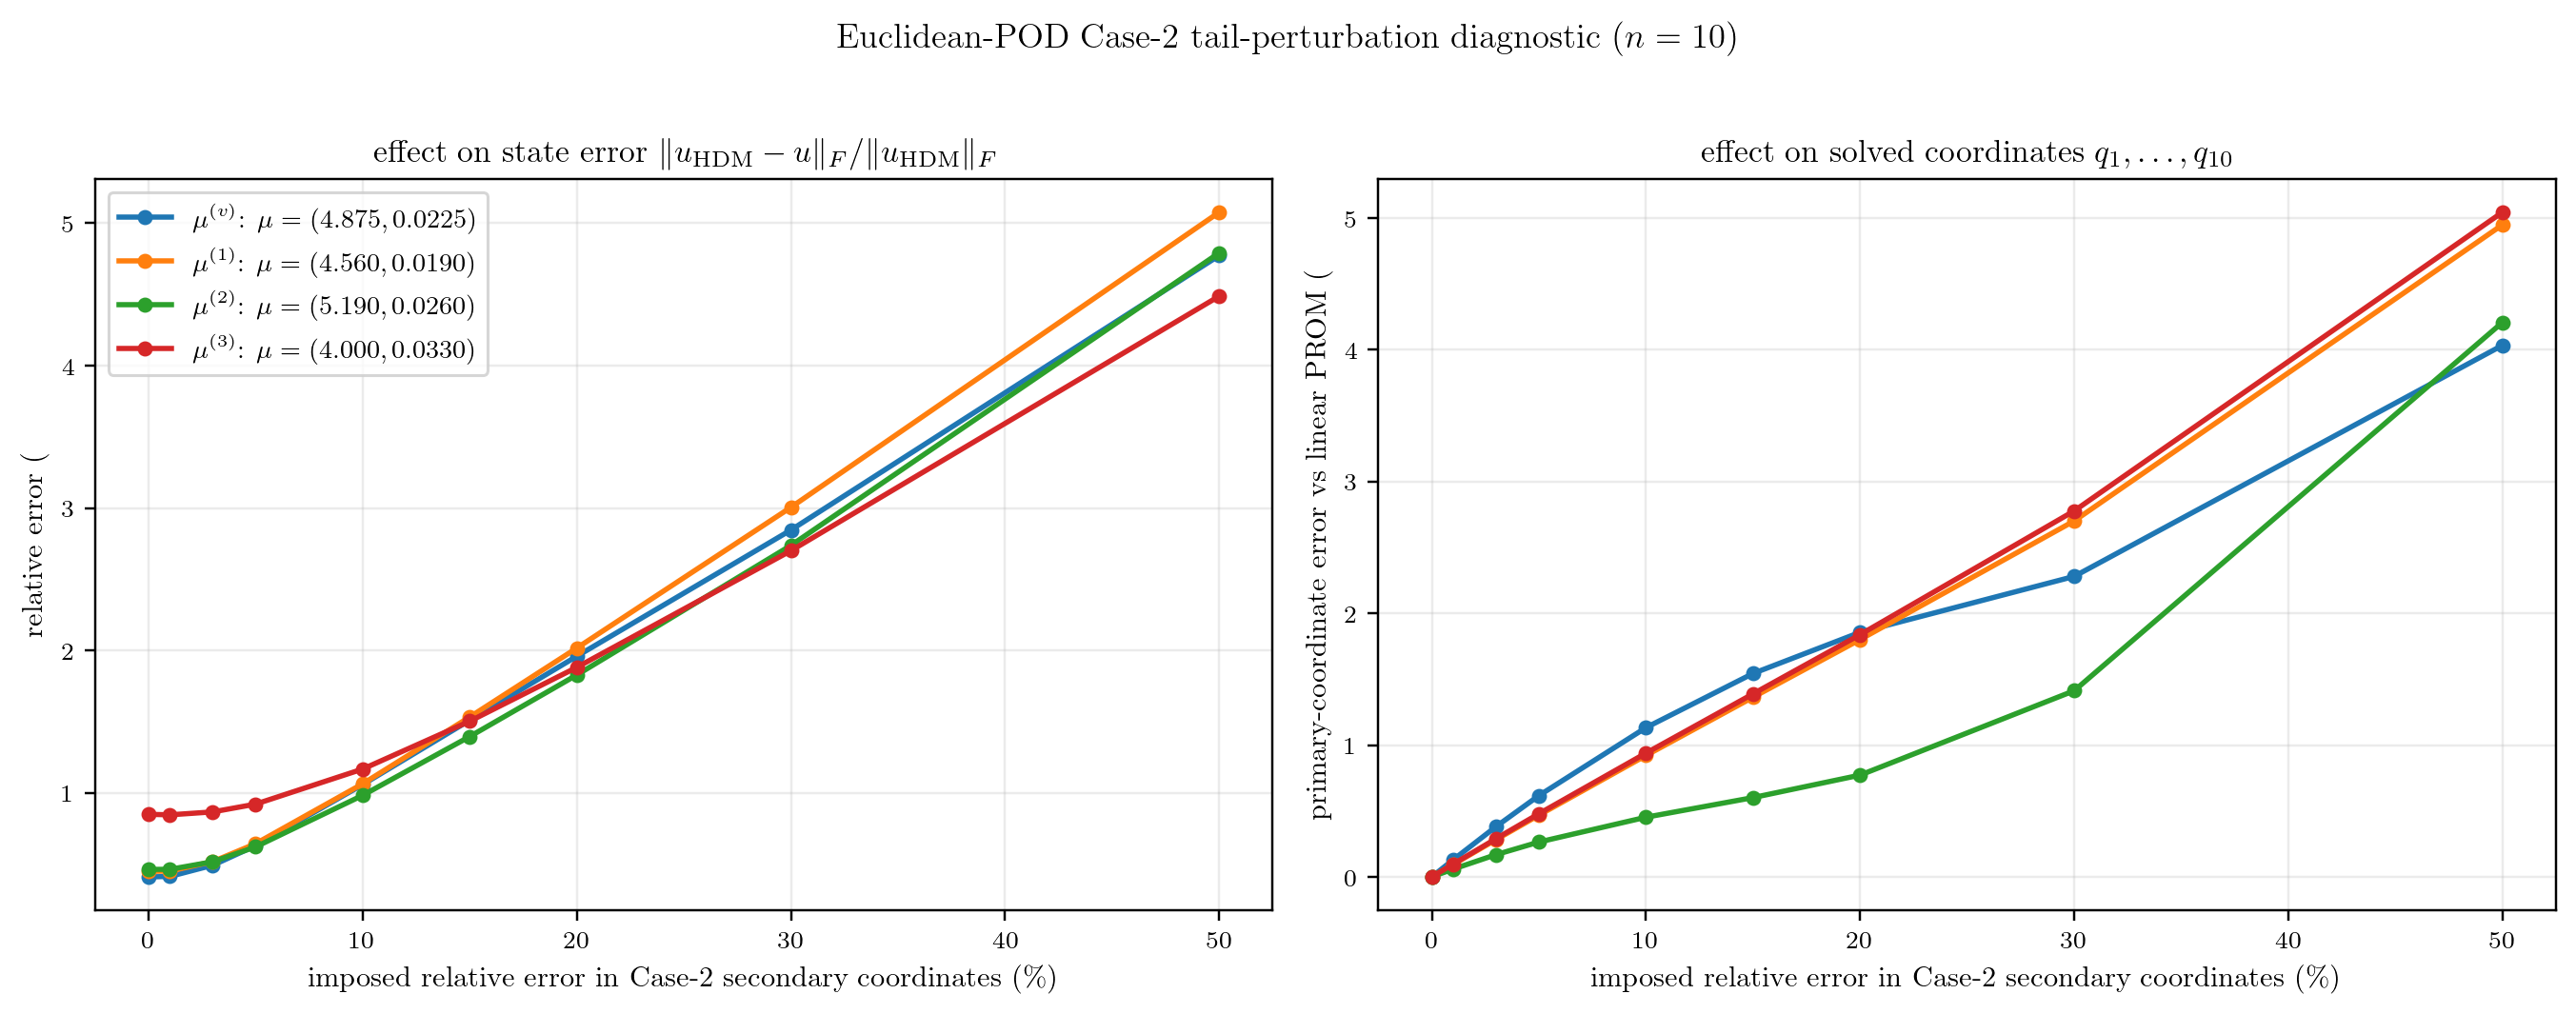
\includegraphics[width=\textwidth]{Figures/euclidean_prom_only/euclidean_prom_case2_tail_sensitivity.png}
\caption{Case--2 sensitivity to a prescribed secondary-tail
error, restricted to perturbations up to $50\%$.  Left: state error against
the HDM.  Right: error in the ten residual-solved primary coordinates against
linear PROM.}
\label{fig:tail-perturbation}
\end{figure}

\clearpage
\section{HPROM Enrichment Details}
\label{app:hprom-details}
Table~\ref{tab:hprom-enrichment-training} reports training and held-out
parameter-validation coordinate errors for the retrained maps.  The
validation trajectories were used for checkpoint selection, not as
independent tests of online state accuracy.
\begin{table}[H]
\centering
\caption{Training and held-out parameter-validation coordinate errors
(\%) for each regression family and data budget.  The POD--NN--ROM row
repeats the errors of the master map shared with HPROM--ANN Case~2, not a separate fit.  These are
not HDM-relative state errors; online size refers to deployment.}
\label{tab:hprom-enrichment-training}
\papertable{tables/euclidean_hprom/training_enrichment.tex}
\end{table}

Tables~\ref{tab:hprom-lhs8-state}, \ref{tab:hprom-lhs12-state}, and
\ref{tab:hprom-lhs18-state}
resolve the in-domain means of Table~\ref{tab:hprom-enrichment-state}
into their three reporting parameters.  All three use the same HDM reference,
model order, and error definition as the main comparison.  The linear HPROM
was not retrained or re-hyperreduced; its fixed reference values are repeated
for comparison.  These are conventional enriched deployments.  The
HPROM--ANN Case~2+$\mathbf B_3$ row is marked with dashes because no
enriched adaptive ECM rule was evaluated.
\begin{table}[H]
\centering
\caption{Pointwise $9+8$ HPROM state-history errors $e_u$ (\%).
The mean averages the three in-domain reporting points; online size
has the same meaning as in the baseline table.}
\label{tab:hprom-lhs8-state}
\papertable{tables/euclidean_hprom/lhs8_state.tex}
\end{table}
\begin{table}[H]
\centering
\caption{Pointwise $9+12$ HPROM state-history errors $e_u$ (\%).
The mean averages the three in-domain reporting points; online size
has the same meaning as in the baseline table.}
\label{tab:hprom-lhs12-state}
\papertable{tables/euclidean_hprom/lhs12_state.tex}
\end{table}
\begin{table}[H]
\centering
\caption{Pointwise $9+18$ HPROM state-history errors $e_u$ (\%).
The mean averages the three in-domain reporting points; online size
has the same meaning as in the baseline table.}
\label{tab:hprom-lhs18-state}
\papertable{tables/euclidean_hprom/lhs18_state.tex}
\end{table}
\clearpage
\section{Alternative Inner Products for POD Basis Construction}
\label{app:lspg-sensitive}
The snapshot SVD in Section~\ref{sec:projection-framework} uses the standard
state inner product.  Other choices can be appropriate for basis construction
while retaining the same trial-map and LSPG structure.  In particular, let
$\mathbf M_u=\mathbf M_u^T\succ0$ define a discrete state inner product,
\begin{equation}
(\mathbf v,\mathbf w)_{\mathbf M_u}=\mathbf v^T\mathbf M_u\mathbf w,
\qquad
\norm{\mathbf v}_{\mathbf M_u}^2=\mathbf v^T\mathbf M_u\mathbf v.
\label{eq:mass-inner-product}
\end{equation}
For finite-element discretizations, $\mathbf M_u$ can be the consistent or
lumped mass matrix.  For finite-volume discretizations, it is commonly the
block-diagonal matrix of cell volumes.  This weighting is particularly
natural on an unstructured mesh, where cells need not represent equal
physical volume.

The corresponding mass-weighted POD can be computed from the snapshot
correlation matrix
\begin{equation}
\mathbf C_M=\mathbf S_c^T\mathbf M_u\mathbf S_c,
\qquad
\mathbf C_M\mathbf y_i=\lambda_i\mathbf y_i,
\label{eq:mass-pod-correlation}
\end{equation}
with modes
\begin{equation}
\boldsymbol\phi_i=\frac{1}{\sqrt{\lambda_i}}\mathbf S_c\mathbf y_i,
\qquad
\boldsymbol\phi_i^T\mathbf M_u\boldsymbol\phi_j=\delta_{ij}.
\label{eq:mass-pod-modes}
\end{equation}
For the resulting metric-orthonormal basis
$\boldsymbol\Phi=[\boldsymbol\phi_1\ \cdots\
\boldsymbol\phi_{n_{\mathrm{tot}}}]$, the corresponding projection
coordinates are
$\boldsymbol\Phi^T\mathbf M_u(\uvec-\uvec_{\mathrm{ref}})$.
Euclidean projection and state/coefficient norm identities must therefore
be replaced by their metric counterparts; the inner product used to
construct the basis does not automatically change the online residual norm.
When all control volumes are equal, $\mathbf M_u$ is a scalar multiple of
the identity and this construction spans the same POD subspaces as the
standard snapshot SVD.  The uniform Cartesian Burgers discretization used
here has precisely this property.

As a separate double check, we also tested a basis metric that combines the
physical mass term with local sensitivity of the time-discrete LSPG residual.
For selected parameter--time states $s\in\mathcal S_{\mathrm{met}}$, define
\begin{equation}
\mathbf G
=\varepsilon\mathbf M_u+
\sum_{s\in\mathcal S_{\mathrm{met}}}
\omega_s\mathbf J_s^T\mathbf P_s\mathbf J_s,
\label{eq:combined-lspg-mass-metric}
\end{equation}
where $\mathbf J_s=\partial\mathbf r_s/\partial\uvec$,
$\mathbf P_s\succeq0$ weights the residual equations, and $\omega_s>0$
weights the selected states.  The full-residual experiment used
$\mathbf P_s=\mathbf I$.  Writing
\begin{equation}
\mathbf C_J=
\sum_{s\in\mathcal S_{\mathrm{met}}}
\omega_s\mathbf S_c^T\mathbf J_s^T\mathbf P_s\mathbf J_s\mathbf S_c,
\qquad
\mathbf C_G=\mathbf S_c^T\mathbf G\mathbf S_c
=\varepsilon\mathbf C_M+\mathbf C_J,
\label{eq:combined-lspg-correlation}
\end{equation}
we scaled the regularization according to
\begin{equation}
\varepsilon=\eta\,
\frac{\operatorname{tr}(\mathbf C_J)}
{\operatorname{tr}(\mathbf C_M)},
\qquad \eta=10^{-10}.
\label{eq:combined-lspg-mass-scale}
\end{equation}
An eigendecomposition of $\mathbf C_G$ then gives modes by the analogue of
\eqref{eq:mass-pod-modes}, with $\mathbf M_u$ replaced by $\mathbf G$.
Thus the sensitivity information affects only basis construction; the online
residual objective and trial-tangent formulas retain their form after the
basis is fixed.  A $\mathbf G$-orthonormal basis does not, however, satisfy
the Euclidean identities in \eqref{eq:partition-orthogonality} unless it is
also reorthonormalized in the standard state inner product.

For this benchmark, the mass-weighted construction and the combined
mass--LSPG-sensitivity construction did not produce a systematic accuracy
advantage in the linear reference, the learned closures, or the controlled
secondary-tail tests.  The differences were small and not consistent across
the evaluated parameter points.  We therefore use the standard Euclidean
snapshot SVD for every result in the paper.  The alternatives above remain
valid options for problems whose spatial discretization or mesh geometry
provides a reason to prefer a different state inner product.

% Citation keys follow Google Scholar-style BibTeX identifiers.
\begin{thebibliography}{99}

\bibitem{hernandez2017dimensional}
J.~A. Hern\'andez, M.~A. Caicedo, A. Ferrer,
Dimensional hyper-reduction of nonlinear finite element models via empirical
cubature, Computer Methods in Applied Mechanics and Engineering 313 (2017)
687--722.

\bibitem{hernandez2020multiscale}
J.~A. Hern\'andez,
A multiscale method for periodic structures using domain decomposition and
ECM-hyperreduction, Computer Methods in Applied Mechanics and Engineering
368 (2020) 113192.

\bibitem{farhat2015structure}
C. Farhat, T. Chapman, P. Avery,
Structure-preserving, stability, and accuracy properties of the
energy-conserving sampling and weighting method for the hyper reduction of
nonlinear finite element dynamic models, International Journal for Numerical
Methods in Engineering 102(5) (2015) 1077--1110.

\bibitem{barnett2023neural}
J. Barnett, C. Farhat, Y. Maday,
Neural-network-augmented projection-based model order reduction for
mitigating the Kolmogorov barrier to reducibility, Journal of Computational
Physics 492 (2023) 112420.

\bibitem{aghili2026nonlinear}
J. Aghili, H. Ballout, Y. Maday, C. Prud'Homme,
Nonlinear compressive reduced basis approximation: when Taylor meets
Kolmogorov, arXiv preprint arXiv:2601.13712 (2026).

\bibitem{chmiel2025unified}
M.~R. Chmiel, J. Barnett, C. Farhat,
Unified LSPG model reduction framework and assessment for hypersonic
computational fluid dynamics, AIAA Journal 63(1) (2025) 72--90.

\bibitem{ares2026closure}
S. Ares De Parga, R. Tezaur, C.~G. Hern\'andez, C. Farhat,
Nonlinear projection-based model order reduction with machine learning
regression for closure error modeling in the latent space, Computer Methods
in Applied Mechanics and Engineering 448 (2026) 118443.

\bibitem{fresca2022pod}
S. Fresca, A. Manzoni,
POD-DL-ROM: Enhancing deep learning-based reduced order models for nonlinear
parametrized PDEs by proper orthogonal decomposition, Computer Methods in
Applied Mechanics and Engineering 388 (2022) 114181.

\bibitem{lee2020model}
K. Lee, K.~T. Carlberg,
Model reduction of dynamical systems on nonlinear manifolds using deep
convolutional autoencoders, Journal of Computational Physics 404 (2020)
108973.

\bibitem{romor2025explicable}
F. Romor, G. Stabile, G. Rozza,
Explicable hyper-reduced order models on nonlinearly approximated solution
manifolds of compressible and incompressible Navier--Stokes equations,
Journal of Computational Physics 524 (2025) 113729.

\bibitem{de2023hyper}
S. Ares De Parga, J.~R. Bravo, J.~A. Hern\'andez, R. Zorrilla, R. Rossi,
Hyper-reduction for Petrov--Galerkin reduced order models, Computer Methods
in Applied Mechanics and Engineering 416 (2023) 116298.

\bibitem{hesthaven2018non}
J.~S. Hesthaven, S. Ubbiali,
Non-intrusive reduced order modeling of nonlinear problems using neural
networks, Journal of Computational Physics 363 (2018) 55--78.

\end{thebibliography}

\end{document}
